% Created by tikzDevice version 0.12.6 on 2025-02-15 08:25:01
% !TEX encoding = UTF-8 Unicode
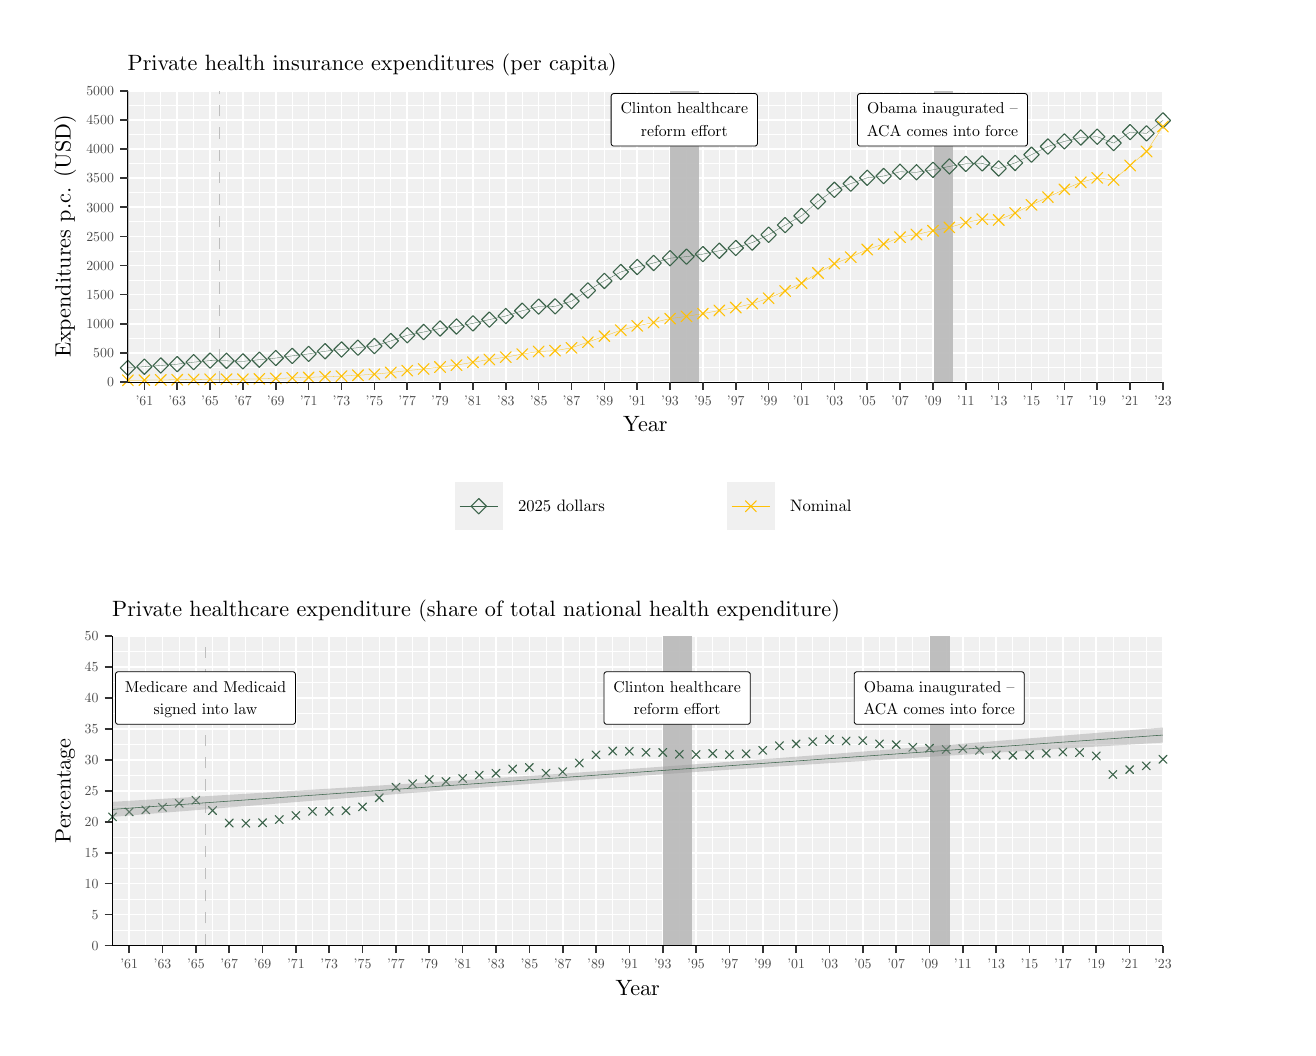
\begin{tikzpicture}[x=1pt,y=1pt]
\definecolor{fillColor}{RGB}{255,255,255}
\path[use as bounding box,fill=fillColor,fill opacity=0.00] (0,0) rectangle (455.30,361.35);
\begin{scope}
\path[clip] (  0.00,164.25) rectangle (455.30,361.35);
\definecolor{drawColor}{RGB}{255,255,255}
\definecolor{fillColor}{RGB}{255,255,255}

\path[draw=drawColor,line width= 0.6pt,line join=round,line cap=round,fill=fillColor] (  0.00,164.25) rectangle (455.30,361.35);
\end{scope}
\begin{scope}
\path[clip] (  0.00,  0.00) rectangle (455.30,361.35);
\definecolor{fillColor}{gray}{0.94}

\path[fill=fillColor] ( 36.14,233.28) rectangle (410.30,338.57);
\definecolor{drawColor}{RGB}{255,255,255}

\path[draw=drawColor,line width= 0.3pt,line join=round] ( 36.14,238.54) --
	(410.30,238.54);

\path[draw=drawColor,line width= 0.3pt,line join=round] ( 36.14,249.07) --
	(410.30,249.07);

\path[draw=drawColor,line width= 0.3pt,line join=round] ( 36.14,259.60) --
	(410.30,259.60);

\path[draw=drawColor,line width= 0.3pt,line join=round] ( 36.14,270.13) --
	(410.30,270.13);

\path[draw=drawColor,line width= 0.3pt,line join=round] ( 36.14,280.66) --
	(410.30,280.66);

\path[draw=drawColor,line width= 0.3pt,line join=round] ( 36.14,291.19) --
	(410.30,291.19);

\path[draw=drawColor,line width= 0.3pt,line join=round] ( 36.14,301.72) --
	(410.30,301.72);

\path[draw=drawColor,line width= 0.3pt,line join=round] ( 36.14,312.25) --
	(410.30,312.25);

\path[draw=drawColor,line width= 0.3pt,line join=round] ( 36.14,322.78) --
	(410.30,322.78);

\path[draw=drawColor,line width= 0.3pt,line join=round] ( 36.14,333.31) --
	(410.30,333.31);

\path[draw=drawColor,line width= 0.3pt,line join=round] ( 36.23,233.28) --
	( 36.23,338.57);

\path[draw=drawColor,line width= 0.3pt,line join=round] ( 48.10,233.28) --
	( 48.10,338.57);

\path[draw=drawColor,line width= 0.3pt,line join=round] ( 59.97,233.28) --
	( 59.97,338.57);

\path[draw=drawColor,line width= 0.3pt,line join=round] ( 71.85,233.28) --
	( 71.85,338.57);

\path[draw=drawColor,line width= 0.3pt,line join=round] ( 83.72,233.28) --
	( 83.72,338.57);

\path[draw=drawColor,line width= 0.3pt,line join=round] ( 95.59,233.28) --
	( 95.59,338.57);

\path[draw=drawColor,line width= 0.3pt,line join=round] (107.46,233.28) --
	(107.46,338.57);

\path[draw=drawColor,line width= 0.3pt,line join=round] (119.34,233.28) --
	(119.34,338.57);

\path[draw=drawColor,line width= 0.3pt,line join=round] (131.21,233.28) --
	(131.21,338.57);

\path[draw=drawColor,line width= 0.3pt,line join=round] (143.08,233.28) --
	(143.08,338.57);

\path[draw=drawColor,line width= 0.3pt,line join=round] (154.96,233.28) --
	(154.96,338.57);

\path[draw=drawColor,line width= 0.3pt,line join=round] (166.83,233.28) --
	(166.83,338.57);

\path[draw=drawColor,line width= 0.3pt,line join=round] (178.70,233.28) --
	(178.70,338.57);

\path[draw=drawColor,line width= 0.3pt,line join=round] (190.58,233.28) --
	(190.58,338.57);

\path[draw=drawColor,line width= 0.3pt,line join=round] (202.45,233.28) --
	(202.45,338.57);

\path[draw=drawColor,line width= 0.3pt,line join=round] (214.32,233.28) --
	(214.32,338.57);

\path[draw=drawColor,line width= 0.3pt,line join=round] (226.19,233.28) --
	(226.19,338.57);

\path[draw=drawColor,line width= 0.3pt,line join=round] (238.07,233.28) --
	(238.07,338.57);

\path[draw=drawColor,line width= 0.3pt,line join=round] (249.94,233.28) --
	(249.94,338.57);

\path[draw=drawColor,line width= 0.3pt,line join=round] (261.81,233.28) --
	(261.81,338.57);

\path[draw=drawColor,line width= 0.3pt,line join=round] (273.69,233.28) --
	(273.69,338.57);

\path[draw=drawColor,line width= 0.3pt,line join=round] (285.56,233.28) --
	(285.56,338.57);

\path[draw=drawColor,line width= 0.3pt,line join=round] (297.43,233.28) --
	(297.43,338.57);

\path[draw=drawColor,line width= 0.3pt,line join=round] (309.30,233.28) --
	(309.30,338.57);

\path[draw=drawColor,line width= 0.3pt,line join=round] (321.18,233.28) --
	(321.18,338.57);

\path[draw=drawColor,line width= 0.3pt,line join=round] (333.05,233.28) --
	(333.05,338.57);

\path[draw=drawColor,line width= 0.3pt,line join=round] (344.92,233.28) --
	(344.92,338.57);

\path[draw=drawColor,line width= 0.3pt,line join=round] (356.80,233.28) --
	(356.80,338.57);

\path[draw=drawColor,line width= 0.3pt,line join=round] (368.67,233.28) --
	(368.67,338.57);

\path[draw=drawColor,line width= 0.3pt,line join=round] (380.54,233.28) --
	(380.54,338.57);

\path[draw=drawColor,line width= 0.3pt,line join=round] (392.41,233.28) --
	(392.41,338.57);

\path[draw=drawColor,line width= 0.3pt,line join=round] (404.29,233.28) --
	(404.29,338.57);

\path[draw=drawColor,line width= 0.6pt,line join=round] ( 36.14,233.28) --
	(410.30,233.28);

\path[draw=drawColor,line width= 0.6pt,line join=round] ( 36.14,243.81) --
	(410.30,243.81);

\path[draw=drawColor,line width= 0.6pt,line join=round] ( 36.14,254.34) --
	(410.30,254.34);

\path[draw=drawColor,line width= 0.6pt,line join=round] ( 36.14,264.87) --
	(410.30,264.87);

\path[draw=drawColor,line width= 0.6pt,line join=round] ( 36.14,275.40) --
	(410.30,275.40);

\path[draw=drawColor,line width= 0.6pt,line join=round] ( 36.14,285.93) --
	(410.30,285.93);

\path[draw=drawColor,line width= 0.6pt,line join=round] ( 36.14,296.46) --
	(410.30,296.46);

\path[draw=drawColor,line width= 0.6pt,line join=round] ( 36.14,306.99) --
	(410.30,306.99);

\path[draw=drawColor,line width= 0.6pt,line join=round] ( 36.14,317.51) --
	(410.30,317.51);

\path[draw=drawColor,line width= 0.6pt,line join=round] ( 36.14,328.04) --
	(410.30,328.04);

\path[draw=drawColor,line width= 0.6pt,line join=round] ( 36.14,338.57) --
	(410.30,338.57);

\path[draw=drawColor,line width= 0.6pt,line join=round] ( 42.17,233.28) --
	( 42.17,338.57);

\path[draw=drawColor,line width= 0.6pt,line join=round] ( 54.03,233.28) --
	( 54.03,338.57);

\path[draw=drawColor,line width= 0.6pt,line join=round] ( 65.91,233.28) --
	( 65.91,338.57);

\path[draw=drawColor,line width= 0.6pt,line join=round] ( 77.78,233.28) --
	( 77.78,338.57);

\path[draw=drawColor,line width= 0.6pt,line join=round] ( 89.66,233.28) --
	( 89.66,338.57);

\path[draw=drawColor,line width= 0.6pt,line join=round] (101.52,233.28) --
	(101.52,338.57);

\path[draw=drawColor,line width= 0.6pt,line join=round] (113.41,233.28) --
	(113.41,338.57);

\path[draw=drawColor,line width= 0.6pt,line join=round] (125.27,233.28) --
	(125.27,338.57);

\path[draw=drawColor,line width= 0.6pt,line join=round] (137.15,233.28) --
	(137.15,338.57);

\path[draw=drawColor,line width= 0.6pt,line join=round] (149.02,233.28) --
	(149.02,338.57);

\path[draw=drawColor,line width= 0.6pt,line join=round] (160.90,233.28) --
	(160.90,338.57);

\path[draw=drawColor,line width= 0.6pt,line join=round] (172.76,233.28) --
	(172.76,338.57);

\path[draw=drawColor,line width= 0.6pt,line join=round] (184.64,233.28) --
	(184.64,338.57);

\path[draw=drawColor,line width= 0.6pt,line join=round] (196.51,233.28) --
	(196.51,338.57);

\path[draw=drawColor,line width= 0.6pt,line join=round] (208.39,233.28) --
	(208.39,338.57);

\path[draw=drawColor,line width= 0.6pt,line join=round] (220.25,233.28) --
	(220.25,338.57);

\path[draw=drawColor,line width= 0.6pt,line join=round] (232.13,233.28) --
	(232.13,338.57);

\path[draw=drawColor,line width= 0.6pt,line join=round] (244.00,233.28) --
	(244.00,338.57);

\path[draw=drawColor,line width= 0.6pt,line join=round] (255.88,233.28) --
	(255.88,338.57);

\path[draw=drawColor,line width= 0.6pt,line join=round] (267.74,233.28) --
	(267.74,338.57);

\path[draw=drawColor,line width= 0.6pt,line join=round] (279.63,233.28) --
	(279.63,338.57);

\path[draw=drawColor,line width= 0.6pt,line join=round] (291.49,233.28) --
	(291.49,338.57);

\path[draw=drawColor,line width= 0.6pt,line join=round] (303.37,233.28) --
	(303.37,338.57);

\path[draw=drawColor,line width= 0.6pt,line join=round] (315.24,233.28) --
	(315.24,338.57);

\path[draw=drawColor,line width= 0.6pt,line join=round] (327.12,233.28) --
	(327.12,338.57);

\path[draw=drawColor,line width= 0.6pt,line join=round] (338.98,233.28) --
	(338.98,338.57);

\path[draw=drawColor,line width= 0.6pt,line join=round] (350.86,233.28) --
	(350.86,338.57);

\path[draw=drawColor,line width= 0.6pt,line join=round] (362.73,233.28) --
	(362.73,338.57);

\path[draw=drawColor,line width= 0.6pt,line join=round] (374.61,233.28) --
	(374.61,338.57);

\path[draw=drawColor,line width= 0.6pt,line join=round] (386.47,233.28) --
	(386.47,338.57);

\path[draw=drawColor,line width= 0.6pt,line join=round] (398.35,233.28) --
	(398.35,338.57);

\path[draw=drawColor,line width= 0.6pt,line join=round] (410.22,233.28) --
	(410.22,338.57);
\definecolor{drawColor}{RGB}{190,190,190}

\path[draw=drawColor,line width= 0.6pt,line join=round] ( 36.22,233.28) -- ( 36.22,338.57);
\definecolor{fillColor}{RGB}{190,190,190}

\path[fill=fillColor,fill opacity=0.01] (232.13,233.28) rectangle (242.42,338.57);

\path[fill=fillColor,fill opacity=0.01] (232.13,233.28) rectangle (242.42,338.57);

\path[fill=fillColor,fill opacity=0.01] (232.13,233.28) rectangle (242.42,338.57);

\path[fill=fillColor,fill opacity=0.01] (232.13,233.28) rectangle (242.42,338.57);

\path[fill=fillColor,fill opacity=0.01] (232.13,233.28) rectangle (242.42,338.57);

\path[fill=fillColor,fill opacity=0.01] (232.13,233.28) rectangle (242.42,338.57);

\path[fill=fillColor,fill opacity=0.01] (232.13,233.28) rectangle (242.42,338.57);

\path[fill=fillColor,fill opacity=0.01] (232.13,233.28) rectangle (242.42,338.57);

\path[fill=fillColor,fill opacity=0.01] (232.13,233.28) rectangle (242.42,338.57);

\path[fill=fillColor,fill opacity=0.01] (232.13,233.28) rectangle (242.42,338.57);

\path[fill=fillColor,fill opacity=0.01] (232.13,233.28) rectangle (242.42,338.57);

\path[fill=fillColor,fill opacity=0.01] (232.13,233.28) rectangle (242.42,338.57);

\path[fill=fillColor,fill opacity=0.01] (232.13,233.28) rectangle (242.42,338.57);

\path[fill=fillColor,fill opacity=0.01] (232.13,233.28) rectangle (242.42,338.57);

\path[fill=fillColor,fill opacity=0.01] (232.13,233.28) rectangle (242.42,338.57);

\path[fill=fillColor,fill opacity=0.01] (232.13,233.28) rectangle (242.42,338.57);

\path[fill=fillColor,fill opacity=0.01] (232.13,233.28) rectangle (242.42,338.57);

\path[fill=fillColor,fill opacity=0.01] (232.13,233.28) rectangle (242.42,338.57);

\path[fill=fillColor,fill opacity=0.01] (232.13,233.28) rectangle (242.42,338.57);

\path[fill=fillColor,fill opacity=0.01] (232.13,233.28) rectangle (242.42,338.57);

\path[fill=fillColor,fill opacity=0.01] (232.13,233.28) rectangle (242.42,338.57);

\path[fill=fillColor,fill opacity=0.01] (232.13,233.28) rectangle (242.42,338.57);

\path[fill=fillColor,fill opacity=0.01] (232.13,233.28) rectangle (242.42,338.57);

\path[fill=fillColor,fill opacity=0.01] (232.13,233.28) rectangle (242.42,338.57);

\path[fill=fillColor,fill opacity=0.01] (232.13,233.28) rectangle (242.42,338.57);

\path[fill=fillColor,fill opacity=0.01] (232.13,233.28) rectangle (242.42,338.57);

\path[fill=fillColor,fill opacity=0.01] (232.13,233.28) rectangle (242.42,338.57);

\path[fill=fillColor,fill opacity=0.01] (232.13,233.28) rectangle (242.42,338.57);

\path[fill=fillColor,fill opacity=0.01] (232.13,233.28) rectangle (242.42,338.57);

\path[fill=fillColor,fill opacity=0.01] (232.13,233.28) rectangle (242.42,338.57);

\path[fill=fillColor,fill opacity=0.01] (232.13,233.28) rectangle (242.42,338.57);

\path[fill=fillColor,fill opacity=0.01] (232.13,233.28) rectangle (242.42,338.57);

\path[fill=fillColor,fill opacity=0.01] (232.13,233.28) rectangle (242.42,338.57);

\path[fill=fillColor,fill opacity=0.01] (232.13,233.28) rectangle (242.42,338.57);

\path[fill=fillColor,fill opacity=0.01] (232.13,233.28) rectangle (242.42,338.57);

\path[fill=fillColor,fill opacity=0.01] (232.13,233.28) rectangle (242.42,338.57);

\path[fill=fillColor,fill opacity=0.01] (232.13,233.28) rectangle (242.42,338.57);

\path[fill=fillColor,fill opacity=0.01] (232.13,233.28) rectangle (242.42,338.57);

\path[fill=fillColor,fill opacity=0.01] (232.13,233.28) rectangle (242.42,338.57);

\path[fill=fillColor,fill opacity=0.01] (232.13,233.28) rectangle (242.42,338.57);

\path[fill=fillColor,fill opacity=0.01] (232.13,233.28) rectangle (242.42,338.57);

\path[fill=fillColor,fill opacity=0.01] (232.13,233.28) rectangle (242.42,338.57);

\path[fill=fillColor,fill opacity=0.01] (232.13,233.28) rectangle (242.42,338.57);

\path[fill=fillColor,fill opacity=0.01] (232.13,233.28) rectangle (242.42,338.57);

\path[fill=fillColor,fill opacity=0.01] (232.13,233.28) rectangle (242.42,338.57);

\path[fill=fillColor,fill opacity=0.01] (232.13,233.28) rectangle (242.42,338.57);

\path[fill=fillColor,fill opacity=0.01] (232.13,233.28) rectangle (242.42,338.57);

\path[fill=fillColor,fill opacity=0.01] (232.13,233.28) rectangle (242.42,338.57);

\path[fill=fillColor,fill opacity=0.01] (232.13,233.28) rectangle (242.42,338.57);

\path[fill=fillColor,fill opacity=0.01] (232.13,233.28) rectangle (242.42,338.57);

\path[fill=fillColor,fill opacity=0.01] (232.13,233.28) rectangle (242.42,338.57);

\path[fill=fillColor,fill opacity=0.01] (232.13,233.28) rectangle (242.42,338.57);

\path[fill=fillColor,fill opacity=0.01] (232.13,233.28) rectangle (242.42,338.57);

\path[fill=fillColor,fill opacity=0.01] (232.13,233.28) rectangle (242.42,338.57);

\path[fill=fillColor,fill opacity=0.01] (232.13,233.28) rectangle (242.42,338.57);

\path[fill=fillColor,fill opacity=0.01] (232.13,233.28) rectangle (242.42,338.57);

\path[fill=fillColor,fill opacity=0.01] (232.13,233.28) rectangle (242.42,338.57);

\path[fill=fillColor,fill opacity=0.01] (232.13,233.28) rectangle (242.42,338.57);

\path[fill=fillColor,fill opacity=0.01] (232.13,233.28) rectangle (242.42,338.57);

\path[fill=fillColor,fill opacity=0.01] (232.13,233.28) rectangle (242.42,338.57);

\path[fill=fillColor,fill opacity=0.01] (232.13,233.28) rectangle (242.42,338.57);

\path[fill=fillColor,fill opacity=0.01] (232.13,233.28) rectangle (242.42,338.57);

\path[fill=fillColor,fill opacity=0.01] (232.13,233.28) rectangle (242.42,338.57);

\path[fill=fillColor,fill opacity=0.01] (232.13,233.28) rectangle (242.42,338.57);

\path[fill=fillColor,fill opacity=0.01] (327.43,233.28) rectangle (334.37,338.57);

\path[fill=fillColor,fill opacity=0.01] (327.43,233.28) rectangle (334.37,338.57);

\path[fill=fillColor,fill opacity=0.01] (327.43,233.28) rectangle (334.37,338.57);

\path[fill=fillColor,fill opacity=0.01] (327.43,233.28) rectangle (334.37,338.57);

\path[fill=fillColor,fill opacity=0.01] (327.43,233.28) rectangle (334.37,338.57);

\path[fill=fillColor,fill opacity=0.01] (327.43,233.28) rectangle (334.37,338.57);

\path[fill=fillColor,fill opacity=0.01] (327.43,233.28) rectangle (334.37,338.57);

\path[fill=fillColor,fill opacity=0.01] (327.43,233.28) rectangle (334.37,338.57);

\path[fill=fillColor,fill opacity=0.01] (327.43,233.28) rectangle (334.37,338.57);

\path[fill=fillColor,fill opacity=0.01] (327.43,233.28) rectangle (334.37,338.57);

\path[fill=fillColor,fill opacity=0.01] (327.43,233.28) rectangle (334.37,338.57);

\path[fill=fillColor,fill opacity=0.01] (327.43,233.28) rectangle (334.37,338.57);

\path[fill=fillColor,fill opacity=0.01] (327.43,233.28) rectangle (334.37,338.57);

\path[fill=fillColor,fill opacity=0.01] (327.43,233.28) rectangle (334.37,338.57);

\path[fill=fillColor,fill opacity=0.01] (327.43,233.28) rectangle (334.37,338.57);

\path[fill=fillColor,fill opacity=0.01] (327.43,233.28) rectangle (334.37,338.57);

\path[fill=fillColor,fill opacity=0.01] (327.43,233.28) rectangle (334.37,338.57);

\path[fill=fillColor,fill opacity=0.01] (327.43,233.28) rectangle (334.37,338.57);

\path[fill=fillColor,fill opacity=0.01] (327.43,233.28) rectangle (334.37,338.57);

\path[fill=fillColor,fill opacity=0.01] (327.43,233.28) rectangle (334.37,338.57);

\path[fill=fillColor,fill opacity=0.01] (327.43,233.28) rectangle (334.37,338.57);

\path[fill=fillColor,fill opacity=0.01] (327.43,233.28) rectangle (334.37,338.57);

\path[fill=fillColor,fill opacity=0.01] (327.43,233.28) rectangle (334.37,338.57);

\path[fill=fillColor,fill opacity=0.01] (327.43,233.28) rectangle (334.37,338.57);

\path[fill=fillColor,fill opacity=0.01] (327.43,233.28) rectangle (334.37,338.57);

\path[fill=fillColor,fill opacity=0.01] (327.43,233.28) rectangle (334.37,338.57);

\path[fill=fillColor,fill opacity=0.01] (327.43,233.28) rectangle (334.37,338.57);

\path[fill=fillColor,fill opacity=0.01] (327.43,233.28) rectangle (334.37,338.57);

\path[fill=fillColor,fill opacity=0.01] (327.43,233.28) rectangle (334.37,338.57);

\path[fill=fillColor,fill opacity=0.01] (327.43,233.28) rectangle (334.37,338.57);

\path[fill=fillColor,fill opacity=0.01] (327.43,233.28) rectangle (334.37,338.57);

\path[fill=fillColor,fill opacity=0.01] (327.43,233.28) rectangle (334.37,338.57);

\path[fill=fillColor,fill opacity=0.01] (327.43,233.28) rectangle (334.37,338.57);

\path[fill=fillColor,fill opacity=0.01] (327.43,233.28) rectangle (334.37,338.57);

\path[fill=fillColor,fill opacity=0.01] (327.43,233.28) rectangle (334.37,338.57);

\path[fill=fillColor,fill opacity=0.01] (327.43,233.28) rectangle (334.37,338.57);

\path[fill=fillColor,fill opacity=0.01] (327.43,233.28) rectangle (334.37,338.57);

\path[fill=fillColor,fill opacity=0.01] (327.43,233.28) rectangle (334.37,338.57);

\path[fill=fillColor,fill opacity=0.01] (327.43,233.28) rectangle (334.37,338.57);

\path[fill=fillColor,fill opacity=0.01] (327.43,233.28) rectangle (334.37,338.57);

\path[fill=fillColor,fill opacity=0.01] (327.43,233.28) rectangle (334.37,338.57);

\path[fill=fillColor,fill opacity=0.01] (327.43,233.28) rectangle (334.37,338.57);

\path[fill=fillColor,fill opacity=0.01] (327.43,233.28) rectangle (334.37,338.57);

\path[fill=fillColor,fill opacity=0.01] (327.43,233.28) rectangle (334.37,338.57);

\path[fill=fillColor,fill opacity=0.01] (327.43,233.28) rectangle (334.37,338.57);

\path[fill=fillColor,fill opacity=0.01] (327.43,233.28) rectangle (334.37,338.57);

\path[fill=fillColor,fill opacity=0.01] (327.43,233.28) rectangle (334.37,338.57);

\path[fill=fillColor,fill opacity=0.01] (327.43,233.28) rectangle (334.37,338.57);

\path[fill=fillColor,fill opacity=0.01] (327.43,233.28) rectangle (334.37,338.57);

\path[fill=fillColor,fill opacity=0.01] (327.43,233.28) rectangle (334.37,338.57);

\path[fill=fillColor,fill opacity=0.01] (327.43,233.28) rectangle (334.37,338.57);

\path[fill=fillColor,fill opacity=0.01] (327.43,233.28) rectangle (334.37,338.57);

\path[fill=fillColor,fill opacity=0.01] (327.43,233.28) rectangle (334.37,338.57);

\path[fill=fillColor,fill opacity=0.01] (327.43,233.28) rectangle (334.37,338.57);

\path[fill=fillColor,fill opacity=0.01] (327.43,233.28) rectangle (334.37,338.57);

\path[fill=fillColor,fill opacity=0.01] (327.43,233.28) rectangle (334.37,338.57);

\path[fill=fillColor,fill opacity=0.01] (327.43,233.28) rectangle (334.37,338.57);

\path[fill=fillColor,fill opacity=0.01] (327.43,233.28) rectangle (334.37,338.57);

\path[fill=fillColor,fill opacity=0.01] (327.43,233.28) rectangle (334.37,338.57);

\path[fill=fillColor,fill opacity=0.01] (327.43,233.28) rectangle (334.37,338.57);

\path[fill=fillColor,fill opacity=0.01] (327.43,233.28) rectangle (334.37,338.57);

\path[fill=fillColor,fill opacity=0.01] (327.43,233.28) rectangle (334.37,338.57);

\path[fill=fillColor,fill opacity=0.01] (327.43,233.28) rectangle (334.37,338.57);

\path[fill=fillColor,fill opacity=0.01] (327.43,233.28) rectangle (334.37,338.57);

\path[draw=drawColor,line width= 0.6pt,dash pattern=on 4pt off 4pt ,line join=round] ( 69.33,233.28) -- ( 69.33,338.57);
\definecolor{drawColor}{RGB}{0,0,0}
\definecolor{fillColor}{RGB}{255,255,255}

\path[draw=drawColor,line width= 0.3pt,line join=round,line cap=round,fill=fillColor] (211.87,318.56) --
	(262.67,318.56) --
	(262.63,318.56) --
	(262.80,318.57) --
	(262.96,318.60) --
	(263.11,318.66) --
	(263.26,318.74) --
	(263.39,318.85) --
	(263.49,318.97) --
	(263.58,319.11) --
	(263.65,319.26) --
	(263.69,319.42) --
	(263.70,319.59) --
	(263.70,319.59) --
	(263.70,336.50) --
	(263.70,336.50) --
	(263.69,336.67) --
	(263.65,336.83) --
	(263.58,336.98) --
	(263.49,337.12) --
	(263.39,337.24) --
	(263.26,337.35) --
	(263.11,337.43) --
	(262.96,337.49) --
	(262.80,337.52) --
	(262.67,337.53) --
	(211.87,337.53) --
	(211.99,337.52) --
	(211.83,337.53) --
	(211.66,337.51) --
	(211.50,337.46) --
	(211.35,337.39) --
	(211.22,337.30) --
	(211.10,337.18) --
	(211.00,337.05) --
	(210.92,336.90) --
	(210.87,336.75) --
	(210.84,336.58) --
	(210.84,336.50) --
	(210.84,319.59) --
	(210.84,319.67) --
	(210.84,319.51) --
	(210.87,319.34) --
	(210.92,319.19) --
	(211.00,319.04) --
	(211.10,318.91) --
	(211.22,318.79) --
	(211.35,318.70) --
	(211.50,318.63) --
	(211.66,318.58) --
	(211.83,318.56) --
	cycle;
\end{scope}
\begin{scope}
\path[clip] (  0.00,  0.00) rectangle (455.30,361.35);
\definecolor{drawColor}{RGB}{0,0,0}

\node[text=drawColor,anchor=base,inner sep=0pt, outer sep=0pt, scale=  0.57] at (237.27,330.18) {Clinton healthcare };

\node[text=drawColor,anchor=base,inner sep=0pt, outer sep=0pt, scale=  0.57] at (237.27,321.99) { reform effort};
\end{scope}
\begin{scope}
\path[clip] (  0.00,  0.00) rectangle (455.30,361.35);
\definecolor{drawColor}{RGB}{0,0,0}
\definecolor{fillColor}{RGB}{255,255,255}

\path[draw=drawColor,line width= 0.3pt,line join=round,line cap=round,fill=fillColor] (300.88,318.56) --
	(360.25,318.56) --
	(360.21,318.56) --
	(360.37,318.57) --
	(360.54,318.60) --
	(360.69,318.66) --
	(360.83,318.74) --
	(360.96,318.85) --
	(361.07,318.97) --
	(361.16,319.11) --
	(361.22,319.26) --
	(361.26,319.42) --
	(361.28,319.59) --
	(361.28,319.59) --
	(361.28,336.50) --
	(361.28,336.50) --
	(361.26,336.67) --
	(361.22,336.83) --
	(361.16,336.98) --
	(361.07,337.12) --
	(360.96,337.24) --
	(360.83,337.35) --
	(360.69,337.43) --
	(360.54,337.49) --
	(360.37,337.52) --
	(360.25,337.53) --
	(300.88,337.53) --
	(301.00,337.52) --
	(300.84,337.53) --
	(300.67,337.51) --
	(300.51,337.46) --
	(300.36,337.39) --
	(300.23,337.30) --
	(300.11,337.18) --
	(300.01,337.05) --
	(299.93,336.90) --
	(299.88,336.75) --
	(299.85,336.58) --
	(299.85,336.50) --
	(299.85,319.59) --
	(299.85,319.67) --
	(299.85,319.51) --
	(299.88,319.34) --
	(299.93,319.19) --
	(300.01,319.04) --
	(300.11,318.91) --
	(300.23,318.79) --
	(300.36,318.70) --
	(300.51,318.63) --
	(300.67,318.58) --
	(300.84,318.56) --
	cycle;
\end{scope}
\begin{scope}
\path[clip] (  0.00,  0.00) rectangle (455.30,361.35);
\definecolor{drawColor}{RGB}{0,0,0}

\node[text=drawColor,anchor=base,inner sep=0pt, outer sep=0pt, scale=  0.57] at (330.56,330.18) {Obama inaugurated -- };

\node[text=drawColor,anchor=base,inner sep=0pt, outer sep=0pt, scale=  0.57] at (330.56,321.99) { ACA comes into force};
\end{scope}
\begin{scope}
\path[clip] (  0.00,  0.00) rectangle (455.30,361.35);
\definecolor{drawColor}{RGB}{60,100,75}

\path[draw=drawColor,line width= 0.4pt,line join=round,line cap=round] ( 33.44,238.42) --
	( 36.22,241.19) --
	( 38.99,238.42) --
	( 36.22,235.64) --
	cycle;

\path[draw=drawColor,line width= 0.4pt,line join=round,line cap=round] ( 39.39,238.84) --
	( 42.17,241.62) --
	( 44.94,238.84) --
	( 42.17,236.07) --
	cycle;

\path[draw=drawColor,line width= 0.4pt,line join=round,line cap=round] ( 45.33,239.28) --
	( 48.10,242.05) --
	( 50.88,239.28) --
	( 48.10,236.50) --
	cycle;

\path[draw=drawColor,line width= 0.4pt,line join=round,line cap=round] ( 51.26,239.76) --
	( 54.03,242.54) --
	( 56.81,239.76) --
	( 54.03,236.99) --
	cycle;

\path[draw=drawColor,line width= 0.4pt,line join=round,line cap=round] ( 57.19,240.48) --
	( 59.97,243.26) --
	( 62.74,240.48) --
	( 59.97,237.71) --
	cycle;

\path[draw=drawColor,line width= 0.4pt,line join=round,line cap=round] ( 63.14,241.04) --
	( 65.91,243.82) --
	( 68.69,241.04) --
	( 65.91,238.27) --
	cycle;

\path[draw=drawColor,line width= 0.4pt,line join=round,line cap=round] ( 69.07,240.96) --
	( 71.85,243.74) --
	( 74.62,240.96) --
	( 71.85,238.19) --
	cycle;

\path[draw=drawColor,line width= 0.4pt,line join=round,line cap=round] ( 75.00,240.77) --
	( 77.78,243.55) --
	( 80.55,240.77) --
	( 77.78,238.00) --
	cycle;

\path[draw=drawColor,line width= 0.4pt,line join=round,line cap=round] ( 80.94,241.37) --
	( 83.71,244.14) --
	( 86.49,241.37) --
	( 83.71,238.60) --
	cycle;

\path[draw=drawColor,line width= 0.4pt,line join=round,line cap=round] ( 86.88,241.96) --
	( 89.66,244.74) --
	( 92.43,241.96) --
	( 89.66,239.19) --
	cycle;

\path[draw=drawColor,line width= 0.4pt,line join=round,line cap=round] ( 92.82,242.75) --
	( 95.59,245.52) --
	( 98.37,242.75) --
	( 95.59,239.97) --
	cycle;

\path[draw=drawColor,line width= 0.4pt,line join=round,line cap=round] ( 98.75,243.47) --
	(101.52,246.25) --
	(104.30,243.47) --
	(101.52,240.70) --
	cycle;

\path[draw=drawColor,line width= 0.4pt,line join=round,line cap=round] (104.68,244.43) --
	(107.46,247.20) --
	(110.23,244.43) --
	(107.46,241.65) --
	cycle;

\path[draw=drawColor,line width= 0.4pt,line join=round,line cap=round] (110.63,245.08) --
	(113.41,247.85) --
	(116.18,245.08) --
	(113.41,242.30) --
	cycle;

\path[draw=drawColor,line width= 0.4pt,line join=round,line cap=round] (116.56,245.71) --
	(119.34,248.49) --
	(122.11,245.71) --
	(119.34,242.94) --
	cycle;

\path[draw=drawColor,line width= 0.4pt,line join=round,line cap=round] (122.50,246.30) --
	(125.27,249.08) --
	(128.05,246.30) --
	(125.27,243.53) --
	cycle;

\path[draw=drawColor,line width= 0.4pt,line join=round,line cap=round] (128.43,248.13) --
	(131.20,250.91) --
	(133.98,248.13) --
	(131.20,245.36) --
	cycle;

\path[draw=drawColor,line width= 0.4pt,line join=round,line cap=round] (134.38,250.20) --
	(137.15,252.98) --
	(139.93,250.20) --
	(137.15,247.43) --
	cycle;

\path[draw=drawColor,line width= 0.4pt,line join=round,line cap=round] (140.31,251.38) --
	(143.08,254.15) --
	(145.86,251.38) --
	(143.08,248.60) --
	cycle;

\path[draw=drawColor,line width= 0.4pt,line join=round,line cap=round] (146.24,252.64) --
	(149.02,255.41) --
	(151.79,252.64) --
	(149.02,249.86) --
	cycle;

\path[draw=drawColor,line width= 0.4pt,line join=round,line cap=round] (152.17,253.35) --
	(154.95,256.13) --
	(157.72,253.35) --
	(154.95,250.58) --
	cycle;

\path[draw=drawColor,line width= 0.4pt,line join=round,line cap=round] (158.12,254.51) --
	(160.90,257.28) --
	(163.67,254.51) --
	(160.90,251.73) --
	cycle;

\path[draw=drawColor,line width= 0.4pt,line join=round,line cap=round] (164.05,255.87) --
	(166.83,258.64) --
	(169.60,255.87) --
	(166.83,253.10) --
	cycle;

\path[draw=drawColor,line width= 0.4pt,line join=round,line cap=round] (169.99,257.15) --
	(172.76,259.92) --
	(175.54,257.15) --
	(172.76,254.37) --
	cycle;

\path[draw=drawColor,line width= 0.4pt,line join=round,line cap=round] (175.92,259.06) --
	(178.69,261.83) --
	(181.47,259.06) --
	(178.69,256.28) --
	cycle;

\path[draw=drawColor,line width= 0.4pt,line join=round,line cap=round] (181.87,260.56) --
	(184.64,263.33) --
	(187.42,260.56) --
	(184.64,257.78) --
	cycle;

\path[draw=drawColor,line width= 0.4pt,line join=round,line cap=round] (187.80,260.65) --
	(190.58,263.42) --
	(193.35,260.65) --
	(190.58,257.87) --
	cycle;

\path[draw=drawColor,line width= 0.4pt,line join=round,line cap=round] (193.73,262.51) --
	(196.51,265.29) --
	(199.28,262.51) --
	(196.51,259.74) --
	cycle;

\path[draw=drawColor,line width= 0.4pt,line join=round,line cap=round] (199.67,266.39) --
	(202.44,269.16) --
	(205.21,266.39) --
	(202.44,263.61) --
	cycle;

\path[draw=drawColor,line width= 0.4pt,line join=round,line cap=round] (205.61,269.83) --
	(208.39,272.60) --
	(211.16,269.83) --
	(208.39,267.05) --
	cycle;

\path[draw=drawColor,line width= 0.4pt,line join=round,line cap=round] (211.55,273.07) --
	(214.32,275.84) --
	(217.10,273.07) --
	(214.32,270.29) --
	cycle;

\path[draw=drawColor,line width= 0.4pt,line join=round,line cap=round] (217.48,274.85) --
	(220.25,277.63) --
	(223.03,274.85) --
	(220.25,272.08) --
	cycle;

\path[draw=drawColor,line width= 0.4pt,line join=round,line cap=round] (223.41,276.32) --
	(226.19,279.09) --
	(228.96,276.32) --
	(226.19,273.54) --
	cycle;

\path[draw=drawColor,line width= 0.4pt,line join=round,line cap=round] (229.36,278.05) --
	(232.13,280.82) --
	(234.91,278.05) --
	(232.13,275.27) --
	cycle;

\path[draw=drawColor,line width= 0.4pt,line join=round,line cap=round] (235.29,278.60) --
	(238.07,281.38) --
	(240.84,278.60) --
	(238.07,275.83) --
	cycle;

\path[draw=drawColor,line width= 0.4pt,line join=round,line cap=round] (241.22,279.53) --
	(244.00,282.31) --
	(246.77,279.53) --
	(244.00,276.76) --
	cycle;

\path[draw=drawColor,line width= 0.4pt,line join=round,line cap=round] (247.16,280.74) --
	(249.93,283.51) --
	(252.71,280.74) --
	(249.93,277.96) --
	cycle;

\path[draw=drawColor,line width= 0.4pt,line join=round,line cap=round] (253.11,281.74) --
	(255.88,284.52) --
	(258.66,281.74) --
	(255.88,278.97) --
	cycle;

\path[draw=drawColor,line width= 0.4pt,line join=round,line cap=round] (259.04,283.68) --
	(261.81,286.46) --
	(264.59,283.68) --
	(261.81,280.91) --
	cycle;

\path[draw=drawColor,line width= 0.4pt,line join=round,line cap=round] (264.97,286.52) --
	(267.74,289.30) --
	(270.52,286.52) --
	(267.74,283.75) --
	cycle;

\path[draw=drawColor,line width= 0.4pt,line join=round,line cap=round] (270.90,290.02) --
	(273.68,292.79) --
	(276.45,290.02) --
	(273.68,287.24) --
	cycle;

\path[draw=drawColor,line width= 0.4pt,line join=round,line cap=round] (276.85,293.35) --
	(279.63,296.13) --
	(282.40,293.35) --
	(279.63,290.58) --
	cycle;

\path[draw=drawColor,line width= 0.4pt,line join=round,line cap=round] (282.78,298.55) --
	(285.56,301.33) --
	(288.33,298.55) --
	(285.56,295.78) --
	cycle;

\path[draw=drawColor,line width= 0.4pt,line join=round,line cap=round] (288.72,302.76) --
	(291.49,305.54) --
	(294.27,302.76) --
	(291.49,299.99) --
	cycle;

\path[draw=drawColor,line width= 0.4pt,line join=round,line cap=round] (294.65,304.98) --
	(297.42,307.75) --
	(300.20,304.98) --
	(297.42,302.20) --
	cycle;

\path[draw=drawColor,line width= 0.4pt,line join=round,line cap=round] (300.60,307.10) --
	(303.37,309.87) --
	(306.15,307.10) --
	(303.37,304.33) --
	cycle;

\path[draw=drawColor,line width= 0.4pt,line join=round,line cap=round] (306.53,307.74) --
	(309.30,310.51) --
	(312.08,307.74) --
	(309.30,304.96) --
	cycle;

\path[draw=drawColor,line width= 0.4pt,line join=round,line cap=round] (312.46,309.27) --
	(315.24,312.04) --
	(318.01,309.27) --
	(315.24,306.49) --
	cycle;

\path[draw=drawColor,line width= 0.4pt,line join=round,line cap=round] (318.39,309.10) --
	(321.17,311.88) --
	(323.94,309.10) --
	(321.17,306.33) --
	cycle;

\path[draw=drawColor,line width= 0.4pt,line join=round,line cap=round] (324.34,309.98) --
	(327.12,312.75) --
	(329.89,309.98) --
	(327.12,307.20) --
	cycle;

\path[draw=drawColor,line width= 0.4pt,line join=round,line cap=round] (330.28,311.23) --
	(333.05,314.00) --
	(335.82,311.23) --
	(333.05,308.45) --
	cycle;

\path[draw=drawColor,line width= 0.4pt,line join=round,line cap=round] (336.21,312.14) --
	(338.98,314.91) --
	(341.76,312.14) --
	(338.98,309.36) --
	cycle;

\path[draw=drawColor,line width= 0.4pt,line join=round,line cap=round] (342.14,312.31) --
	(344.91,315.08) --
	(347.69,312.31) --
	(344.91,309.53) --
	cycle;

\path[draw=drawColor,line width= 0.4pt,line join=round,line cap=round] (348.09,310.47) --
	(350.86,313.24) --
	(353.64,310.47) --
	(350.86,307.69) --
	cycle;

\path[draw=drawColor,line width= 0.4pt,line join=round,line cap=round] (354.02,312.47) --
	(356.80,315.24) --
	(359.57,312.47) --
	(356.80,309.69) --
	cycle;

\path[draw=drawColor,line width= 0.4pt,line join=round,line cap=round] (359.95,315.46) --
	(362.73,318.23) --
	(365.50,315.46) --
	(362.73,312.68) --
	cycle;

\path[draw=drawColor,line width= 0.4pt,line join=round,line cap=round] (365.89,318.40) --
	(368.66,321.17) --
	(371.44,318.40) --
	(368.66,315.62) --
	cycle;

\path[draw=drawColor,line width= 0.4pt,line join=round,line cap=round] (371.83,320.26) --
	(374.61,323.03) --
	(377.38,320.26) --
	(374.61,317.48) --
	cycle;

\path[draw=drawColor,line width= 0.4pt,line join=round,line cap=round] (377.77,321.65) --
	(380.54,324.43) --
	(383.32,321.65) --
	(380.54,318.88) --
	cycle;

\path[draw=drawColor,line width= 0.4pt,line join=round,line cap=round] (383.70,321.95) --
	(386.47,324.73) --
	(389.25,321.95) --
	(386.47,319.18) --
	cycle;

\path[draw=drawColor,line width= 0.4pt,line join=round,line cap=round] (389.63,319.64) --
	(392.41,322.42) --
	(395.18,319.64) --
	(392.41,316.87) --
	cycle;

\path[draw=drawColor,line width= 0.4pt,line join=round,line cap=round] (395.58,323.61) --
	(398.35,326.39) --
	(401.13,323.61) --
	(398.35,320.84) --
	cycle;

\path[draw=drawColor,line width= 0.4pt,line join=round,line cap=round] (401.51,323.16) --
	(404.29,325.94) --
	(407.06,323.16) --
	(404.29,320.39) --
	cycle;

\path[draw=drawColor,line width= 0.4pt,line join=round,line cap=round] (407.44,327.84) --
	(410.22,330.62) --
	(412.99,327.84) --
	(410.22,325.07) --
	cycle;
\definecolor{drawColor}{RGB}{255,193,7}

\path[draw=drawColor,line width= 0.4pt,line join=round,line cap=round] ( 34.26,231.96) -- ( 38.18,235.88);

\path[draw=drawColor,line width= 0.4pt,line join=round,line cap=round] ( 34.26,235.88) -- ( 38.18,231.96);

\path[draw=drawColor,line width= 0.4pt,line join=round,line cap=round] ( 40.21,232.02) -- ( 44.13,235.94);

\path[draw=drawColor,line width= 0.4pt,line join=round,line cap=round] ( 40.21,235.94) -- ( 44.13,232.02);

\path[draw=drawColor,line width= 0.4pt,line join=round,line cap=round] ( 46.14,232.08) -- ( 50.06,236.00);

\path[draw=drawColor,line width= 0.4pt,line join=round,line cap=round] ( 46.14,236.00) -- ( 50.06,232.08);

\path[draw=drawColor,line width= 0.4pt,line join=round,line cap=round] ( 52.07,232.15) -- ( 55.99,236.07);

\path[draw=drawColor,line width= 0.4pt,line join=round,line cap=round] ( 52.07,236.07) -- ( 55.99,232.15);

\path[draw=drawColor,line width= 0.4pt,line join=round,line cap=round] ( 58.00,232.26) -- ( 61.93,236.18);

\path[draw=drawColor,line width= 0.4pt,line join=round,line cap=round] ( 58.00,236.18) -- ( 61.93,232.26);

\path[draw=drawColor,line width= 0.4pt,line join=round,line cap=round] ( 63.95,232.35) -- ( 67.88,236.27);

\path[draw=drawColor,line width= 0.4pt,line join=round,line cap=round] ( 63.95,236.27) -- ( 67.88,232.35);

\path[draw=drawColor,line width= 0.4pt,line join=round,line cap=round] ( 69.88,232.36) -- ( 73.81,236.28);

\path[draw=drawColor,line width= 0.4pt,line join=round,line cap=round] ( 69.88,236.28) -- ( 73.81,232.36);

\path[draw=drawColor,line width= 0.4pt,line join=round,line cap=round] ( 75.82,232.36) -- ( 79.74,236.29);

\path[draw=drawColor,line width= 0.4pt,line join=round,line cap=round] ( 75.82,236.29) -- ( 79.74,232.36);

\path[draw=drawColor,line width= 0.4pt,line join=round,line cap=round] ( 81.75,232.49) -- ( 85.67,236.41);

\path[draw=drawColor,line width= 0.4pt,line join=round,line cap=round] ( 81.75,236.41) -- ( 85.67,232.49);

\path[draw=drawColor,line width= 0.4pt,line join=round,line cap=round] ( 87.70,232.63) -- ( 91.62,236.56);

\path[draw=drawColor,line width= 0.4pt,line join=round,line cap=round] ( 87.70,236.56) -- ( 91.62,232.63);

\path[draw=drawColor,line width= 0.4pt,line join=round,line cap=round] ( 93.63,232.83) -- ( 97.55,236.75);

\path[draw=drawColor,line width= 0.4pt,line join=round,line cap=round] ( 93.63,236.75) -- ( 97.55,232.83);

\path[draw=drawColor,line width= 0.4pt,line join=round,line cap=round] ( 99.56,233.03) -- (103.49,236.95);

\path[draw=drawColor,line width= 0.4pt,line join=round,line cap=round] ( 99.56,236.95) -- (103.49,233.03);

\path[draw=drawColor,line width= 0.4pt,line join=round,line cap=round] (105.49,233.28) -- (109.42,237.20);

\path[draw=drawColor,line width= 0.4pt,line join=round,line cap=round] (105.49,237.20) -- (109.42,233.28);

\path[draw=drawColor,line width= 0.4pt,line join=round,line cap=round] (111.44,233.48) -- (115.37,237.40);

\path[draw=drawColor,line width= 0.4pt,line join=round,line cap=round] (111.44,237.40) -- (115.37,233.48);

\path[draw=drawColor,line width= 0.4pt,line join=round,line cap=round] (117.38,233.77) -- (121.30,237.69);

\path[draw=drawColor,line width= 0.4pt,line join=round,line cap=round] (117.38,237.69) -- (121.30,233.77);

\path[draw=drawColor,line width= 0.4pt,line join=round,line cap=round] (123.31,234.16) -- (127.23,238.09);

\path[draw=drawColor,line width= 0.4pt,line join=round,line cap=round] (123.31,238.09) -- (127.23,234.16);

\path[draw=drawColor,line width= 0.4pt,line join=round,line cap=round] (129.24,234.76) -- (133.16,238.69);

\path[draw=drawColor,line width= 0.4pt,line join=round,line cap=round] (129.24,238.69) -- (133.16,234.76);

\path[draw=drawColor,line width= 0.4pt,line join=round,line cap=round] (135.19,235.47) -- (139.11,239.39);

\path[draw=drawColor,line width= 0.4pt,line join=round,line cap=round] (135.19,239.39) -- (139.11,235.47);

\path[draw=drawColor,line width= 0.4pt,line join=round,line cap=round] (141.12,236.04) -- (145.05,239.97);

\path[draw=drawColor,line width= 0.4pt,line join=round,line cap=round] (141.12,239.97) -- (145.05,236.04);

\path[draw=drawColor,line width= 0.4pt,line join=round,line cap=round] (147.05,236.76) -- (150.98,240.68);

\path[draw=drawColor,line width= 0.4pt,line join=round,line cap=round] (147.05,240.68) -- (150.98,236.76);

\path[draw=drawColor,line width= 0.4pt,line join=round,line cap=round] (152.99,237.46) -- (156.91,241.38);

\path[draw=drawColor,line width= 0.4pt,line join=round,line cap=round] (152.99,241.38) -- (156.91,237.46);

\path[draw=drawColor,line width= 0.4pt,line join=round,line cap=round] (158.93,238.48) -- (162.86,242.40);

\path[draw=drawColor,line width= 0.4pt,line join=round,line cap=round] (158.93,242.40) -- (162.86,238.48);

\path[draw=drawColor,line width= 0.4pt,line join=round,line cap=round] (164.87,239.48) -- (168.79,243.41);

\path[draw=drawColor,line width= 0.4pt,line join=round,line cap=round] (164.87,243.41) -- (168.79,239.48);

\path[draw=drawColor,line width= 0.4pt,line join=round,line cap=round] (170.80,240.34) -- (174.72,244.26);

\path[draw=drawColor,line width= 0.4pt,line join=round,line cap=round] (170.80,244.26) -- (174.72,240.34);

\path[draw=drawColor,line width= 0.4pt,line join=round,line cap=round] (176.73,241.42) -- (180.66,245.34);

\path[draw=drawColor,line width= 0.4pt,line join=round,line cap=round] (176.73,245.34) -- (180.66,241.42);

\path[draw=drawColor,line width= 0.4pt,line join=round,line cap=round] (182.68,242.38) -- (186.60,246.30);

\path[draw=drawColor,line width= 0.4pt,line join=round,line cap=round] (182.68,246.30) -- (186.60,242.38);

\path[draw=drawColor,line width= 0.4pt,line join=round,line cap=round] (188.61,242.67) -- (192.54,246.60);

\path[draw=drawColor,line width= 0.4pt,line join=round,line cap=round] (188.61,246.60) -- (192.54,242.67);

\path[draw=drawColor,line width= 0.4pt,line join=round,line cap=round] (194.55,243.69) -- (198.47,247.61);

\path[draw=drawColor,line width= 0.4pt,line join=round,line cap=round] (194.55,247.61) -- (198.47,243.69);

\path[draw=drawColor,line width= 0.4pt,line join=round,line cap=round] (200.48,245.76) -- (204.40,249.68);

\path[draw=drawColor,line width= 0.4pt,line join=round,line cap=round] (200.48,249.68) -- (204.40,245.76);

\path[draw=drawColor,line width= 0.4pt,line join=round,line cap=round] (206.43,247.92) -- (210.35,251.84);

\path[draw=drawColor,line width= 0.4pt,line join=round,line cap=round] (206.43,251.84) -- (210.35,247.92);

\path[draw=drawColor,line width= 0.4pt,line join=round,line cap=round] (212.36,250.05) -- (216.28,253.97);

\path[draw=drawColor,line width= 0.4pt,line join=round,line cap=round] (212.36,253.97) -- (216.28,250.05);

\path[draw=drawColor,line width= 0.4pt,line join=round,line cap=round] (218.29,251.62) -- (222.22,255.55);

\path[draw=drawColor,line width= 0.4pt,line join=round,line cap=round] (218.29,255.55) -- (222.22,251.62);

\path[draw=drawColor,line width= 0.4pt,line join=round,line cap=round] (224.22,252.86) -- (228.15,256.79);

\path[draw=drawColor,line width= 0.4pt,line join=round,line cap=round] (224.22,256.79) -- (228.15,252.86);

\path[draw=drawColor,line width= 0.4pt,line join=round,line cap=round] (230.17,254.26) -- (234.10,258.18);

\path[draw=drawColor,line width= 0.4pt,line join=round,line cap=round] (230.17,258.18) -- (234.10,254.26);

\path[draw=drawColor,line width= 0.4pt,line join=round,line cap=round] (236.10,255.06) -- (240.03,258.99);

\path[draw=drawColor,line width= 0.4pt,line join=round,line cap=round] (236.10,258.99) -- (240.03,255.06);

\path[draw=drawColor,line width= 0.4pt,line join=round,line cap=round] (242.04,256.07) -- (245.96,259.99);

\path[draw=drawColor,line width= 0.4pt,line join=round,line cap=round] (242.04,259.99) -- (245.96,256.07);

\path[draw=drawColor,line width= 0.4pt,line join=round,line cap=round] (247.97,257.21) -- (251.89,261.13);

\path[draw=drawColor,line width= 0.4pt,line join=round,line cap=round] (247.97,261.13) -- (251.89,257.21);

\path[draw=drawColor,line width= 0.4pt,line join=round,line cap=round] (253.92,258.26) -- (257.84,262.18);

\path[draw=drawColor,line width= 0.4pt,line join=round,line cap=round] (253.92,262.18) -- (257.84,258.26);

\path[draw=drawColor,line width= 0.4pt,line join=round,line cap=round] (259.85,259.65) -- (263.77,263.57);

\path[draw=drawColor,line width= 0.4pt,line join=round,line cap=round] (259.85,263.57) -- (263.77,259.65);

\path[draw=drawColor,line width= 0.4pt,line join=round,line cap=round] (265.78,261.63) -- (269.71,265.55);

\path[draw=drawColor,line width= 0.4pt,line join=round,line cap=round] (265.78,265.55) -- (269.71,261.63);

\path[draw=drawColor,line width= 0.4pt,line join=round,line cap=round] (271.72,264.25) -- (275.64,268.17);

\path[draw=drawColor,line width= 0.4pt,line join=round,line cap=round] (271.72,268.17) -- (275.64,264.25);

\path[draw=drawColor,line width= 0.4pt,line join=round,line cap=round] (277.66,267.04) -- (281.59,270.96);

\path[draw=drawColor,line width= 0.4pt,line join=round,line cap=round] (277.66,270.96) -- (281.59,267.04);

\path[draw=drawColor,line width= 0.4pt,line join=round,line cap=round] (283.60,270.76) -- (287.52,274.68);

\path[draw=drawColor,line width= 0.4pt,line join=round,line cap=round] (283.60,274.68) -- (287.52,270.76);

\path[draw=drawColor,line width= 0.4pt,line join=round,line cap=round] (289.53,274.11) -- (293.45,278.03);

\path[draw=drawColor,line width= 0.4pt,line join=round,line cap=round] (289.53,278.03) -- (293.45,274.11);

\path[draw=drawColor,line width= 0.4pt,line join=round,line cap=round] (295.46,276.47) -- (299.39,280.39);

\path[draw=drawColor,line width= 0.4pt,line join=round,line cap=round] (295.46,280.39) -- (299.39,276.47);

\path[draw=drawColor,line width= 0.4pt,line join=round,line cap=round] (301.41,279.22) -- (305.33,283.15);

\path[draw=drawColor,line width= 0.4pt,line join=round,line cap=round] (301.41,283.15) -- (305.33,279.22);

\path[draw=drawColor,line width= 0.4pt,line join=round,line cap=round] (307.34,281.19) -- (311.27,285.11);

\path[draw=drawColor,line width= 0.4pt,line join=round,line cap=round] (307.34,285.11) -- (311.27,281.19);

\path[draw=drawColor,line width= 0.4pt,line join=round,line cap=round] (313.27,283.69) -- (317.20,287.61);

\path[draw=drawColor,line width= 0.4pt,line join=round,line cap=round] (313.27,287.61) -- (317.20,283.69);

\path[draw=drawColor,line width= 0.4pt,line join=round,line cap=round] (319.21,284.64) -- (323.13,288.56);

\path[draw=drawColor,line width= 0.4pt,line join=round,line cap=round] (319.21,288.56) -- (323.13,284.64);

\path[draw=drawColor,line width= 0.4pt,line join=round,line cap=round] (325.16,286.01) -- (329.08,289.94);

\path[draw=drawColor,line width= 0.4pt,line join=round,line cap=round] (325.16,289.94) -- (329.08,286.01);

\path[draw=drawColor,line width= 0.4pt,line join=round,line cap=round] (331.09,287.21) -- (335.01,291.14);

\path[draw=drawColor,line width= 0.4pt,line join=round,line cap=round] (331.09,291.14) -- (335.01,287.21);

\path[draw=drawColor,line width= 0.4pt,line join=round,line cap=round] (337.02,288.94) -- (340.94,292.86);

\path[draw=drawColor,line width= 0.4pt,line join=round,line cap=round] (337.02,292.86) -- (340.94,288.94);

\path[draw=drawColor,line width= 0.4pt,line join=round,line cap=round] (342.95,290.21) -- (346.88,294.13);

\path[draw=drawColor,line width= 0.4pt,line join=round,line cap=round] (342.95,294.13) -- (346.88,290.21);

\path[draw=drawColor,line width= 0.4pt,line join=round,line cap=round] (348.90,289.91) -- (352.83,293.84);

\path[draw=drawColor,line width= 0.4pt,line join=round,line cap=round] (348.90,293.84) -- (352.83,289.91);

\path[draw=drawColor,line width= 0.4pt,line join=round,line cap=round] (354.83,292.41) -- (358.76,296.33);

\path[draw=drawColor,line width= 0.4pt,line join=round,line cap=round] (354.83,296.33) -- (358.76,292.41);

\path[draw=drawColor,line width= 0.4pt,line join=round,line cap=round] (360.77,295.36) -- (364.69,299.29);

\path[draw=drawColor,line width= 0.4pt,line join=round,line cap=round] (360.77,299.29) -- (364.69,295.36);

\path[draw=drawColor,line width= 0.4pt,line join=round,line cap=round] (366.70,298.15) -- (370.62,302.08);

\path[draw=drawColor,line width= 0.4pt,line join=round,line cap=round] (366.70,302.08) -- (370.62,298.15);

\path[draw=drawColor,line width= 0.4pt,line join=round,line cap=round] (372.65,300.94) -- (376.57,304.87);

\path[draw=drawColor,line width= 0.4pt,line join=round,line cap=round] (372.65,304.87) -- (376.57,300.94);

\path[draw=drawColor,line width= 0.4pt,line join=round,line cap=round] (378.58,303.50) -- (382.50,307.43);

\path[draw=drawColor,line width= 0.4pt,line join=round,line cap=round] (378.58,307.43) -- (382.50,303.50);

\path[draw=drawColor,line width= 0.4pt,line join=round,line cap=round] (384.51,305.11) -- (388.44,309.04);

\path[draw=drawColor,line width= 0.4pt,line join=round,line cap=round] (384.51,309.04) -- (388.44,305.11);

\path[draw=drawColor,line width= 0.4pt,line join=round,line cap=round] (390.44,304.35) -- (394.37,308.27);

\path[draw=drawColor,line width= 0.4pt,line join=round,line cap=round] (390.44,308.27) -- (394.37,304.35);

\path[draw=drawColor,line width= 0.4pt,line join=round,line cap=round] (396.39,309.59) -- (400.32,313.52);

\path[draw=drawColor,line width= 0.4pt,line join=round,line cap=round] (396.39,313.52) -- (400.32,309.59);

\path[draw=drawColor,line width= 0.4pt,line join=round,line cap=round] (402.33,314.65) -- (406.25,318.58);

\path[draw=drawColor,line width= 0.4pt,line join=round,line cap=round] (402.33,318.58) -- (406.25,314.65);

\path[draw=drawColor,line width= 0.4pt,line join=round,line cap=round] (408.26,323.66) -- (412.18,327.59);

\path[draw=drawColor,line width= 0.4pt,line join=round,line cap=round] (408.26,327.59) -- (412.18,323.66);

\path[draw=drawColor,line width= 0.1pt,line join=round] ( 36.22,233.92) --
	( 42.17,233.98) --
	( 48.10,234.04) --
	( 54.03,234.11) --
	( 59.97,234.22) --
	( 65.91,234.31) --
	( 71.85,234.32) --
	( 77.78,234.32) --
	( 83.71,234.45) --
	( 89.66,234.59) --
	( 95.59,234.79) --
	(101.52,234.99) --
	(107.46,235.24) --
	(113.41,235.44) --
	(119.34,235.73) --
	(125.27,236.12) --
	(131.20,236.72) --
	(137.15,237.43) --
	(143.08,238.00) --
	(149.02,238.72) --
	(154.95,239.42) --
	(160.90,240.44) --
	(166.83,241.44) --
	(172.76,242.30) --
	(178.69,243.38) --
	(184.64,244.34) --
	(190.58,244.64) --
	(196.51,245.65) --
	(202.44,247.72) --
	(208.39,249.88) --
	(214.32,252.01) --
	(220.25,253.58) --
	(226.19,254.83) --
	(232.13,256.22) --
	(238.07,257.02) --
	(244.00,258.03) --
	(249.93,259.17) --
	(255.88,260.22) --
	(261.81,261.61) --
	(267.74,263.59) --
	(273.68,266.21) --
	(279.63,269.00) --
	(285.56,272.72) --
	(291.49,276.07) --
	(297.42,278.43) --
	(303.37,281.19) --
	(309.30,283.15) --
	(315.24,285.65) --
	(321.17,286.60) --
	(327.12,287.97) --
	(333.05,289.17) --
	(338.98,290.90) --
	(344.91,292.17) --
	(350.86,291.88) --
	(356.80,294.37) --
	(362.73,297.33) --
	(368.66,300.12) --
	(374.61,302.90) --
	(380.54,305.46) --
	(386.47,307.07) --
	(392.41,306.31) --
	(398.35,311.55) --
	(404.29,316.61) --
	(410.22,325.63);
\definecolor{drawColor}{RGB}{60,100,75}

\path[draw=drawColor,line width= 0.1pt,line join=round] ( 36.22,238.42) --
	( 42.17,238.84) --
	( 48.10,239.28) --
	( 54.03,239.76) --
	( 59.97,240.48) --
	( 65.91,241.04) --
	( 71.85,240.96) --
	( 77.78,240.77) --
	( 83.71,241.37) --
	( 89.66,241.96) --
	( 95.59,242.75) --
	(101.52,243.47) --
	(107.46,244.43) --
	(113.41,245.08) --
	(119.34,245.71) --
	(125.27,246.30) --
	(131.20,248.13) --
	(137.15,250.20) --
	(143.08,251.38) --
	(149.02,252.64) --
	(154.95,253.35) --
	(160.90,254.51) --
	(166.83,255.87) --
	(172.76,257.15) --
	(178.69,259.06) --
	(184.64,260.56) --
	(190.58,260.65) --
	(196.51,262.51) --
	(202.44,266.39) --
	(208.39,269.83) --
	(214.32,273.07) --
	(220.25,274.85) --
	(226.19,276.32) --
	(232.13,278.05) --
	(238.07,278.60) --
	(244.00,279.53) --
	(249.93,280.74) --
	(255.88,281.74) --
	(261.81,283.68) --
	(267.74,286.52) --
	(273.68,290.02) --
	(279.63,293.35) --
	(285.56,298.55) --
	(291.49,302.76) --
	(297.42,304.98) --
	(303.37,307.10) --
	(309.30,307.74) --
	(315.24,309.27) --
	(321.17,309.10) --
	(327.12,309.98) --
	(333.05,311.23) --
	(338.98,312.14) --
	(344.91,312.31) --
	(350.86,310.47) --
	(356.80,312.47) --
	(362.73,315.46) --
	(368.66,318.40) --
	(374.61,320.26) --
	(380.54,321.65) --
	(386.47,321.95) --
	(392.41,319.64) --
	(398.35,323.61) --
	(404.29,323.16) --
	(410.22,327.84);
\end{scope}
\begin{scope}
\path[clip] (  0.00,  0.00) rectangle (455.30,361.35);
\definecolor{drawColor}{RGB}{0,0,0}

\path[draw=drawColor,line width= 0.2pt,line join=round] ( 36.14,233.28) --
	( 36.14,338.57);
\end{scope}
\begin{scope}
\path[clip] (  0.00,  0.00) rectangle (455.30,361.35);
\definecolor{drawColor}{gray}{0.30}

\node[text=drawColor,anchor=base east,inner sep=0pt, outer sep=0pt, scale=  0.50] at ( 31.19,231.56) {0};

\node[text=drawColor,anchor=base east,inner sep=0pt, outer sep=0pt, scale=  0.50] at ( 31.19,242.09) {500};

\node[text=drawColor,anchor=base east,inner sep=0pt, outer sep=0pt, scale=  0.50] at ( 31.19,252.62) {1000};

\node[text=drawColor,anchor=base east,inner sep=0pt, outer sep=0pt, scale=  0.50] at ( 31.19,263.15) {1500};

\node[text=drawColor,anchor=base east,inner sep=0pt, outer sep=0pt, scale=  0.50] at ( 31.19,273.67) {2000};

\node[text=drawColor,anchor=base east,inner sep=0pt, outer sep=0pt, scale=  0.50] at ( 31.19,284.20) {2500};

\node[text=drawColor,anchor=base east,inner sep=0pt, outer sep=0pt, scale=  0.50] at ( 31.19,294.73) {3000};

\node[text=drawColor,anchor=base east,inner sep=0pt, outer sep=0pt, scale=  0.50] at ( 31.19,305.26) {3500};

\node[text=drawColor,anchor=base east,inner sep=0pt, outer sep=0pt, scale=  0.50] at ( 31.19,315.79) {4000};

\node[text=drawColor,anchor=base east,inner sep=0pt, outer sep=0pt, scale=  0.50] at ( 31.19,326.32) {4500};

\node[text=drawColor,anchor=base east,inner sep=0pt, outer sep=0pt, scale=  0.50] at ( 31.19,336.85) {5000};
\end{scope}
\begin{scope}
\path[clip] (  0.00,  0.00) rectangle (455.30,361.35);
\definecolor{drawColor}{gray}{0.20}

\path[draw=drawColor,line width= 0.6pt,line join=round] ( 33.39,233.28) --
	( 36.14,233.28);

\path[draw=drawColor,line width= 0.6pt,line join=round] ( 33.39,243.81) --
	( 36.14,243.81);

\path[draw=drawColor,line width= 0.6pt,line join=round] ( 33.39,254.34) --
	( 36.14,254.34);

\path[draw=drawColor,line width= 0.6pt,line join=round] ( 33.39,264.87) --
	( 36.14,264.87);

\path[draw=drawColor,line width= 0.6pt,line join=round] ( 33.39,275.40) --
	( 36.14,275.40);

\path[draw=drawColor,line width= 0.6pt,line join=round] ( 33.39,285.93) --
	( 36.14,285.93);

\path[draw=drawColor,line width= 0.6pt,line join=round] ( 33.39,296.46) --
	( 36.14,296.46);

\path[draw=drawColor,line width= 0.6pt,line join=round] ( 33.39,306.99) --
	( 36.14,306.99);

\path[draw=drawColor,line width= 0.6pt,line join=round] ( 33.39,317.51) --
	( 36.14,317.51);

\path[draw=drawColor,line width= 0.6pt,line join=round] ( 33.39,328.04) --
	( 36.14,328.04);

\path[draw=drawColor,line width= 0.6pt,line join=round] ( 33.39,338.57) --
	( 36.14,338.57);
\end{scope}
\begin{scope}
\path[clip] (  0.00,  0.00) rectangle (455.30,361.35);
\definecolor{drawColor}{RGB}{0,0,0}

\path[draw=drawColor,line width= 0.2pt,line join=round] ( 36.14,233.28) --
	(410.30,233.28);
\end{scope}
\begin{scope}
\path[clip] (  0.00,  0.00) rectangle (455.30,361.35);
\definecolor{drawColor}{gray}{0.20}

\path[draw=drawColor,line width= 0.6pt,line join=round] ( 42.17,230.53) --
	( 42.17,233.28);

\path[draw=drawColor,line width= 0.6pt,line join=round] ( 54.03,230.53) --
	( 54.03,233.28);

\path[draw=drawColor,line width= 0.6pt,line join=round] ( 65.91,230.53) --
	( 65.91,233.28);

\path[draw=drawColor,line width= 0.6pt,line join=round] ( 77.78,230.53) --
	( 77.78,233.28);

\path[draw=drawColor,line width= 0.6pt,line join=round] ( 89.66,230.53) --
	( 89.66,233.28);

\path[draw=drawColor,line width= 0.6pt,line join=round] (101.52,230.53) --
	(101.52,233.28);

\path[draw=drawColor,line width= 0.6pt,line join=round] (113.41,230.53) --
	(113.41,233.28);

\path[draw=drawColor,line width= 0.6pt,line join=round] (125.27,230.53) --
	(125.27,233.28);

\path[draw=drawColor,line width= 0.6pt,line join=round] (137.15,230.53) --
	(137.15,233.28);

\path[draw=drawColor,line width= 0.6pt,line join=round] (149.02,230.53) --
	(149.02,233.28);

\path[draw=drawColor,line width= 0.6pt,line join=round] (160.90,230.53) --
	(160.90,233.28);

\path[draw=drawColor,line width= 0.6pt,line join=round] (172.76,230.53) --
	(172.76,233.28);

\path[draw=drawColor,line width= 0.6pt,line join=round] (184.64,230.53) --
	(184.64,233.28);

\path[draw=drawColor,line width= 0.6pt,line join=round] (196.51,230.53) --
	(196.51,233.28);

\path[draw=drawColor,line width= 0.6pt,line join=round] (208.39,230.53) --
	(208.39,233.28);

\path[draw=drawColor,line width= 0.6pt,line join=round] (220.25,230.53) --
	(220.25,233.28);

\path[draw=drawColor,line width= 0.6pt,line join=round] (232.13,230.53) --
	(232.13,233.28);

\path[draw=drawColor,line width= 0.6pt,line join=round] (244.00,230.53) --
	(244.00,233.28);

\path[draw=drawColor,line width= 0.6pt,line join=round] (255.88,230.53) --
	(255.88,233.28);

\path[draw=drawColor,line width= 0.6pt,line join=round] (267.74,230.53) --
	(267.74,233.28);

\path[draw=drawColor,line width= 0.6pt,line join=round] (279.63,230.53) --
	(279.63,233.28);

\path[draw=drawColor,line width= 0.6pt,line join=round] (291.49,230.53) --
	(291.49,233.28);

\path[draw=drawColor,line width= 0.6pt,line join=round] (303.37,230.53) --
	(303.37,233.28);

\path[draw=drawColor,line width= 0.6pt,line join=round] (315.24,230.53) --
	(315.24,233.28);

\path[draw=drawColor,line width= 0.6pt,line join=round] (327.12,230.53) --
	(327.12,233.28);

\path[draw=drawColor,line width= 0.6pt,line join=round] (338.98,230.53) --
	(338.98,233.28);

\path[draw=drawColor,line width= 0.6pt,line join=round] (350.86,230.53) --
	(350.86,233.28);

\path[draw=drawColor,line width= 0.6pt,line join=round] (362.73,230.53) --
	(362.73,233.28);

\path[draw=drawColor,line width= 0.6pt,line join=round] (374.61,230.53) --
	(374.61,233.28);

\path[draw=drawColor,line width= 0.6pt,line join=round] (386.47,230.53) --
	(386.47,233.28);

\path[draw=drawColor,line width= 0.6pt,line join=round] (398.35,230.53) --
	(398.35,233.28);

\path[draw=drawColor,line width= 0.6pt,line join=round] (410.22,230.53) --
	(410.22,233.28);
\end{scope}
\begin{scope}
\path[clip] (  0.00,  0.00) rectangle (455.30,361.35);
\definecolor{drawColor}{gray}{0.30}

\node[text=drawColor,anchor=base,inner sep=0pt, outer sep=0pt, scale=  0.50] at ( 42.17,224.89) {'61};

\node[text=drawColor,anchor=base,inner sep=0pt, outer sep=0pt, scale=  0.50] at ( 54.03,224.89) {'63};

\node[text=drawColor,anchor=base,inner sep=0pt, outer sep=0pt, scale=  0.50] at ( 65.91,224.89) {'65};

\node[text=drawColor,anchor=base,inner sep=0pt, outer sep=0pt, scale=  0.50] at ( 77.78,224.89) {'67};

\node[text=drawColor,anchor=base,inner sep=0pt, outer sep=0pt, scale=  0.50] at ( 89.66,224.89) {'69};

\node[text=drawColor,anchor=base,inner sep=0pt, outer sep=0pt, scale=  0.50] at (101.52,224.89) {'71};

\node[text=drawColor,anchor=base,inner sep=0pt, outer sep=0pt, scale=  0.50] at (113.41,224.89) {'73};

\node[text=drawColor,anchor=base,inner sep=0pt, outer sep=0pt, scale=  0.50] at (125.27,224.89) {'75};

\node[text=drawColor,anchor=base,inner sep=0pt, outer sep=0pt, scale=  0.50] at (137.15,224.89) {'77};

\node[text=drawColor,anchor=base,inner sep=0pt, outer sep=0pt, scale=  0.50] at (149.02,224.89) {'79};

\node[text=drawColor,anchor=base,inner sep=0pt, outer sep=0pt, scale=  0.50] at (160.90,224.89) {'81};

\node[text=drawColor,anchor=base,inner sep=0pt, outer sep=0pt, scale=  0.50] at (172.76,224.89) {'83};

\node[text=drawColor,anchor=base,inner sep=0pt, outer sep=0pt, scale=  0.50] at (184.64,224.89) {'85};

\node[text=drawColor,anchor=base,inner sep=0pt, outer sep=0pt, scale=  0.50] at (196.51,224.89) {'87};

\node[text=drawColor,anchor=base,inner sep=0pt, outer sep=0pt, scale=  0.50] at (208.39,224.89) {'89};

\node[text=drawColor,anchor=base,inner sep=0pt, outer sep=0pt, scale=  0.50] at (220.25,224.89) {'91};

\node[text=drawColor,anchor=base,inner sep=0pt, outer sep=0pt, scale=  0.50] at (232.13,224.89) {'93};

\node[text=drawColor,anchor=base,inner sep=0pt, outer sep=0pt, scale=  0.50] at (244.00,224.89) {'95};

\node[text=drawColor,anchor=base,inner sep=0pt, outer sep=0pt, scale=  0.50] at (255.88,224.89) {'97};

\node[text=drawColor,anchor=base,inner sep=0pt, outer sep=0pt, scale=  0.50] at (267.74,224.89) {'99};

\node[text=drawColor,anchor=base,inner sep=0pt, outer sep=0pt, scale=  0.50] at (279.63,224.89) {'01};

\node[text=drawColor,anchor=base,inner sep=0pt, outer sep=0pt, scale=  0.50] at (291.49,224.89) {'03};

\node[text=drawColor,anchor=base,inner sep=0pt, outer sep=0pt, scale=  0.50] at (303.37,224.89) {'05};

\node[text=drawColor,anchor=base,inner sep=0pt, outer sep=0pt, scale=  0.50] at (315.24,224.89) {'07};

\node[text=drawColor,anchor=base,inner sep=0pt, outer sep=0pt, scale=  0.50] at (327.12,224.89) {'09};

\node[text=drawColor,anchor=base,inner sep=0pt, outer sep=0pt, scale=  0.50] at (338.98,224.89) {'11};

\node[text=drawColor,anchor=base,inner sep=0pt, outer sep=0pt, scale=  0.50] at (350.86,224.89) {'13};

\node[text=drawColor,anchor=base,inner sep=0pt, outer sep=0pt, scale=  0.50] at (362.73,224.89) {'15};

\node[text=drawColor,anchor=base,inner sep=0pt, outer sep=0pt, scale=  0.50] at (374.61,224.89) {'17};

\node[text=drawColor,anchor=base,inner sep=0pt, outer sep=0pt, scale=  0.50] at (386.47,224.89) {'19};

\node[text=drawColor,anchor=base,inner sep=0pt, outer sep=0pt, scale=  0.50] at (398.35,224.89) {'21};

\node[text=drawColor,anchor=base,inner sep=0pt, outer sep=0pt, scale=  0.50] at (410.22,224.89) {'23};
\end{scope}
\begin{scope}
\path[clip] (  0.00,  0.00) rectangle (455.30,361.35);
\definecolor{drawColor}{RGB}{0,0,0}

\node[text=drawColor,anchor=base,inner sep=0pt, outer sep=0pt, scale=  0.80] at (223.22,215.36) {Year};
\end{scope}
\begin{scope}
\path[clip] (  0.00,  0.00) rectangle (455.30,361.35);
\definecolor{drawColor}{RGB}{0,0,0}

\node[text=drawColor,rotate= 90.00,anchor=base,inner sep=0pt, outer sep=0pt, scale=  0.80] at ( 15.51,285.93) {Expenditures p.c. (USD)};
\end{scope}
\begin{scope}
\path[clip] (  0.00,  0.00) rectangle (455.30,361.35);
\definecolor{fillColor}{RGB}{255,255,255}

\path[fill=fillColor] (143.34,174.25) rectangle (303.10,202.59);
\end{scope}
\begin{scope}
\path[clip] (  0.00,  0.00) rectangle (455.30,361.35);
\definecolor{fillColor}{gray}{0.94}

\path[fill=fillColor] (154.34,179.75) rectangle (171.69,197.09);
\end{scope}
\begin{scope}
\path[clip] (  0.00,  0.00) rectangle (455.30,361.35);
\definecolor{drawColor}{RGB}{60,100,75}

\path[draw=drawColor,line width= 0.4pt,line join=round,line cap=round] (160.24,188.42) --
	(163.01,191.20) --
	(165.79,188.42) --
	(163.01,185.65) --
	cycle;
\end{scope}
\begin{scope}
\path[clip] (  0.00,  0.00) rectangle (455.30,361.35);
\definecolor{drawColor}{RGB}{60,100,75}

\path[draw=drawColor,line width= 0.1pt,line join=round] (156.08,188.42) -- (169.95,188.42);
\end{scope}
\begin{scope}
\path[clip] (  0.00,  0.00) rectangle (455.30,361.35);
\definecolor{fillColor}{gray}{0.94}

\path[fill=fillColor] (252.67,179.75) rectangle (270.01,197.09);
\end{scope}
\begin{scope}
\path[clip] (  0.00,  0.00) rectangle (455.30,361.35);
\definecolor{drawColor}{RGB}{255,193,7}

\path[draw=drawColor,line width= 0.4pt,line join=round,line cap=round] (259.38,186.46) -- (263.30,190.38);

\path[draw=drawColor,line width= 0.4pt,line join=round,line cap=round] (259.38,190.38) -- (263.30,186.46);
\end{scope}
\begin{scope}
\path[clip] (  0.00,  0.00) rectangle (455.30,361.35);
\definecolor{drawColor}{RGB}{255,193,7}

\path[draw=drawColor,line width= 0.1pt,line join=round] (254.40,188.42) -- (268.28,188.42);
\end{scope}
\begin{scope}
\path[clip] (  0.00,  0.00) rectangle (455.30,361.35);
\definecolor{drawColor}{RGB}{0,0,0}

\node[text=drawColor,anchor=base west,inner sep=0pt, outer sep=0pt, scale=  0.60] at (177.19,186.36) {2025 dollars};
\end{scope}
\begin{scope}
\path[clip] (  0.00,  0.00) rectangle (455.30,361.35);
\definecolor{drawColor}{RGB}{0,0,0}

\node[text=drawColor,anchor=base west,inner sep=0pt, outer sep=0pt, scale=  0.60] at (275.51,186.36) {Nominal};
\end{scope}
\begin{scope}
\path[clip] (  0.00,  0.00) rectangle (455.30,361.35);
\definecolor{drawColor}{RGB}{0,0,0}

\node[text=drawColor,anchor=base west,inner sep=0pt, outer sep=0pt, scale=  0.80] at ( 36.14,345.84) {Private health insurance expenditures (per capita)};
\end{scope}
\begin{scope}
\path[clip] (  0.00,  0.00) rectangle (455.30,164.25);
\definecolor{drawColor}{RGB}{255,255,255}
\definecolor{fillColor}{RGB}{255,255,255}

\path[draw=drawColor,line width= 0.6pt,line join=round,line cap=round,fill=fillColor] (  0.00,  0.00) rectangle (455.30,164.25);
\end{scope}
\begin{scope}
\path[clip] (  0.00,  0.00) rectangle (455.30,361.35);
\definecolor{fillColor}{gray}{0.94}

\path[fill=fillColor] ( 30.56, 29.68) rectangle (410.30,141.47);
\definecolor{drawColor}{RGB}{255,255,255}

\path[draw=drawColor,line width= 0.3pt,line join=round] ( 30.56, 35.27) --
	(410.30, 35.27);

\path[draw=drawColor,line width= 0.3pt,line join=round] ( 30.56, 46.45) --
	(410.30, 46.45);

\path[draw=drawColor,line width= 0.3pt,line join=round] ( 30.56, 57.63) --
	(410.30, 57.63);

\path[draw=drawColor,line width= 0.3pt,line join=round] ( 30.56, 68.81) --
	(410.30, 68.81);

\path[draw=drawColor,line width= 0.3pt,line join=round] ( 30.56, 79.99) --
	(410.30, 79.99);

\path[draw=drawColor,line width= 0.3pt,line join=round] ( 30.56, 91.17) --
	(410.30, 91.17);

\path[draw=drawColor,line width= 0.3pt,line join=round] ( 30.56,102.35) --
	(410.30,102.35);

\path[draw=drawColor,line width= 0.3pt,line join=round] ( 30.56,113.53) --
	(410.30,113.53);

\path[draw=drawColor,line width= 0.3pt,line join=round] ( 30.56,124.71) --
	(410.30,124.71);

\path[draw=drawColor,line width= 0.3pt,line join=round] ( 30.56,135.88) --
	(410.30,135.88);

\path[draw=drawColor,line width= 0.3pt,line join=round] ( 30.65, 29.68) --
	( 30.65,141.47);

\path[draw=drawColor,line width= 0.3pt,line join=round] ( 42.70, 29.68) --
	( 42.70,141.47);

\path[draw=drawColor,line width= 0.3pt,line join=round] ( 54.75, 29.68) --
	( 54.75,141.47);

\path[draw=drawColor,line width= 0.3pt,line join=round] ( 66.80, 29.68) --
	( 66.80,141.47);

\path[draw=drawColor,line width= 0.3pt,line join=round] ( 78.85, 29.68) --
	( 78.85,141.47);

\path[draw=drawColor,line width= 0.3pt,line join=round] ( 90.90, 29.68) --
	( 90.90,141.47);

\path[draw=drawColor,line width= 0.3pt,line join=round] (102.95, 29.68) --
	(102.95,141.47);

\path[draw=drawColor,line width= 0.3pt,line join=round] (115.00, 29.68) --
	(115.00,141.47);

\path[draw=drawColor,line width= 0.3pt,line join=round] (127.05, 29.68) --
	(127.05,141.47);

\path[draw=drawColor,line width= 0.3pt,line join=round] (139.10, 29.68) --
	(139.10,141.47);

\path[draw=drawColor,line width= 0.3pt,line join=round] (151.15, 29.68) --
	(151.15,141.47);

\path[draw=drawColor,line width= 0.3pt,line join=round] (163.20, 29.68) --
	(163.20,141.47);

\path[draw=drawColor,line width= 0.3pt,line join=round] (175.25, 29.68) --
	(175.25,141.47);

\path[draw=drawColor,line width= 0.3pt,line join=round] (187.30, 29.68) --
	(187.30,141.47);

\path[draw=drawColor,line width= 0.3pt,line join=round] (199.35, 29.68) --
	(199.35,141.47);

\path[draw=drawColor,line width= 0.3pt,line join=round] (211.40, 29.68) --
	(211.40,141.47);

\path[draw=drawColor,line width= 0.3pt,line join=round] (223.45, 29.68) --
	(223.45,141.47);

\path[draw=drawColor,line width= 0.3pt,line join=round] (235.50, 29.68) --
	(235.50,141.47);

\path[draw=drawColor,line width= 0.3pt,line join=round] (247.55, 29.68) --
	(247.55,141.47);

\path[draw=drawColor,line width= 0.3pt,line join=round] (259.60, 29.68) --
	(259.60,141.47);

\path[draw=drawColor,line width= 0.3pt,line join=round] (271.65, 29.68) --
	(271.65,141.47);

\path[draw=drawColor,line width= 0.3pt,line join=round] (283.70, 29.68) --
	(283.70,141.47);

\path[draw=drawColor,line width= 0.3pt,line join=round] (295.75, 29.68) --
	(295.75,141.47);

\path[draw=drawColor,line width= 0.3pt,line join=round] (307.80, 29.68) --
	(307.80,141.47);

\path[draw=drawColor,line width= 0.3pt,line join=round] (319.85, 29.68) --
	(319.85,141.47);

\path[draw=drawColor,line width= 0.3pt,line join=round] (331.90, 29.68) --
	(331.90,141.47);

\path[draw=drawColor,line width= 0.3pt,line join=round] (343.95, 29.68) --
	(343.95,141.47);

\path[draw=drawColor,line width= 0.3pt,line join=round] (356.00, 29.68) --
	(356.00,141.47);

\path[draw=drawColor,line width= 0.3pt,line join=round] (368.05, 29.68) --
	(368.05,141.47);

\path[draw=drawColor,line width= 0.3pt,line join=round] (380.10, 29.68) --
	(380.10,141.47);

\path[draw=drawColor,line width= 0.3pt,line join=round] (392.15, 29.68) --
	(392.15,141.47);

\path[draw=drawColor,line width= 0.3pt,line join=round] (404.20, 29.68) --
	(404.20,141.47);

\path[draw=drawColor,line width= 0.6pt,line join=round] ( 30.56, 29.68) --
	(410.30, 29.68);

\path[draw=drawColor,line width= 0.6pt,line join=round] ( 30.56, 40.86) --
	(410.30, 40.86);

\path[draw=drawColor,line width= 0.6pt,line join=round] ( 30.56, 52.04) --
	(410.30, 52.04);

\path[draw=drawColor,line width= 0.6pt,line join=round] ( 30.56, 63.22) --
	(410.30, 63.22);

\path[draw=drawColor,line width= 0.6pt,line join=round] ( 30.56, 74.40) --
	(410.30, 74.40);

\path[draw=drawColor,line width= 0.6pt,line join=round] ( 30.56, 85.58) --
	(410.30, 85.58);

\path[draw=drawColor,line width= 0.6pt,line join=round] ( 30.56, 96.76) --
	(410.30, 96.76);

\path[draw=drawColor,line width= 0.6pt,line join=round] ( 30.56,107.94) --
	(410.30,107.94);

\path[draw=drawColor,line width= 0.6pt,line join=round] ( 30.56,119.12) --
	(410.30,119.12);

\path[draw=drawColor,line width= 0.6pt,line join=round] ( 30.56,130.29) --
	(410.30,130.29);

\path[draw=drawColor,line width= 0.6pt,line join=round] ( 30.56,141.47) --
	(410.30,141.47);

\path[draw=drawColor,line width= 0.6pt,line join=round] ( 36.68, 29.68) --
	( 36.68,141.47);

\path[draw=drawColor,line width= 0.6pt,line join=round] ( 48.72, 29.68) --
	( 48.72,141.47);

\path[draw=drawColor,line width= 0.6pt,line join=round] ( 60.78, 29.68) --
	( 60.78,141.47);

\path[draw=drawColor,line width= 0.6pt,line join=round] ( 72.82, 29.68) --
	( 72.82,141.47);

\path[draw=drawColor,line width= 0.6pt,line join=round] ( 84.88, 29.68) --
	( 84.88,141.47);

\path[draw=drawColor,line width= 0.6pt,line join=round] ( 96.92, 29.68) --
	( 96.92,141.47);

\path[draw=drawColor,line width= 0.6pt,line join=round] (108.98, 29.68) --
	(108.98,141.47);

\path[draw=drawColor,line width= 0.6pt,line join=round] (121.02, 29.68) --
	(121.02,141.47);

\path[draw=drawColor,line width= 0.6pt,line join=round] (133.08, 29.68) --
	(133.08,141.47);

\path[draw=drawColor,line width= 0.6pt,line join=round] (145.12, 29.68) --
	(145.12,141.47);

\path[draw=drawColor,line width= 0.6pt,line join=round] (157.18, 29.68) --
	(157.18,141.47);

\path[draw=drawColor,line width= 0.6pt,line join=round] (169.22, 29.68) --
	(169.22,141.47);

\path[draw=drawColor,line width= 0.6pt,line join=round] (181.28, 29.68) --
	(181.28,141.47);

\path[draw=drawColor,line width= 0.6pt,line join=round] (193.32, 29.68) --
	(193.32,141.47);

\path[draw=drawColor,line width= 0.6pt,line join=round] (205.38, 29.68) --
	(205.38,141.47);

\path[draw=drawColor,line width= 0.6pt,line join=round] (217.42, 29.68) --
	(217.42,141.47);

\path[draw=drawColor,line width= 0.6pt,line join=round] (229.48, 29.68) --
	(229.48,141.47);

\path[draw=drawColor,line width= 0.6pt,line join=round] (241.52, 29.68) --
	(241.52,141.47);

\path[draw=drawColor,line width= 0.6pt,line join=round] (253.58, 29.68) --
	(253.58,141.47);

\path[draw=drawColor,line width= 0.6pt,line join=round] (265.62, 29.68) --
	(265.62,141.47);

\path[draw=drawColor,line width= 0.6pt,line join=round] (277.68, 29.68) --
	(277.68,141.47);

\path[draw=drawColor,line width= 0.6pt,line join=round] (289.72, 29.68) --
	(289.72,141.47);

\path[draw=drawColor,line width= 0.6pt,line join=round] (301.78, 29.68) --
	(301.78,141.47);

\path[draw=drawColor,line width= 0.6pt,line join=round] (313.82, 29.68) --
	(313.82,141.47);

\path[draw=drawColor,line width= 0.6pt,line join=round] (325.88, 29.68) --
	(325.88,141.47);

\path[draw=drawColor,line width= 0.6pt,line join=round] (337.92, 29.68) --
	(337.92,141.47);

\path[draw=drawColor,line width= 0.6pt,line join=round] (349.98, 29.68) --
	(349.98,141.47);

\path[draw=drawColor,line width= 0.6pt,line join=round] (362.02, 29.68) --
	(362.02,141.47);

\path[draw=drawColor,line width= 0.6pt,line join=round] (374.08, 29.68) --
	(374.08,141.47);

\path[draw=drawColor,line width= 0.6pt,line join=round] (386.12, 29.68) --
	(386.12,141.47);

\path[draw=drawColor,line width= 0.6pt,line join=round] (398.18, 29.68) --
	(398.18,141.47);

\path[draw=drawColor,line width= 0.6pt,line join=round] (410.22, 29.68) --
	(410.22,141.47);
\definecolor{drawColor}{RGB}{190,190,190}

\path[draw=drawColor,line width= 0.6pt,line join=round] ( 30.64, 29.68) -- ( 30.64,141.47);
\definecolor{fillColor}{RGB}{190,190,190}

\path[fill=fillColor,fill opacity=0.01] (229.48, 29.68) rectangle (239.92,141.47);

\path[fill=fillColor,fill opacity=0.01] (229.48, 29.68) rectangle (239.92,141.47);

\path[fill=fillColor,fill opacity=0.01] (229.48, 29.68) rectangle (239.92,141.47);

\path[fill=fillColor,fill opacity=0.01] (229.48, 29.68) rectangle (239.92,141.47);

\path[fill=fillColor,fill opacity=0.01] (229.48, 29.68) rectangle (239.92,141.47);

\path[fill=fillColor,fill opacity=0.01] (229.48, 29.68) rectangle (239.92,141.47);

\path[fill=fillColor,fill opacity=0.01] (229.48, 29.68) rectangle (239.92,141.47);

\path[fill=fillColor,fill opacity=0.01] (229.48, 29.68) rectangle (239.92,141.47);

\path[fill=fillColor,fill opacity=0.01] (229.48, 29.68) rectangle (239.92,141.47);

\path[fill=fillColor,fill opacity=0.01] (229.48, 29.68) rectangle (239.92,141.47);

\path[fill=fillColor,fill opacity=0.01] (229.48, 29.68) rectangle (239.92,141.47);

\path[fill=fillColor,fill opacity=0.01] (229.48, 29.68) rectangle (239.92,141.47);

\path[fill=fillColor,fill opacity=0.01] (229.48, 29.68) rectangle (239.92,141.47);

\path[fill=fillColor,fill opacity=0.01] (229.48, 29.68) rectangle (239.92,141.47);

\path[fill=fillColor,fill opacity=0.01] (229.48, 29.68) rectangle (239.92,141.47);

\path[fill=fillColor,fill opacity=0.01] (229.48, 29.68) rectangle (239.92,141.47);

\path[fill=fillColor,fill opacity=0.01] (229.48, 29.68) rectangle (239.92,141.47);

\path[fill=fillColor,fill opacity=0.01] (229.48, 29.68) rectangle (239.92,141.47);

\path[fill=fillColor,fill opacity=0.01] (229.48, 29.68) rectangle (239.92,141.47);

\path[fill=fillColor,fill opacity=0.01] (229.48, 29.68) rectangle (239.92,141.47);

\path[fill=fillColor,fill opacity=0.01] (229.48, 29.68) rectangle (239.92,141.47);

\path[fill=fillColor,fill opacity=0.01] (229.48, 29.68) rectangle (239.92,141.47);

\path[fill=fillColor,fill opacity=0.01] (229.48, 29.68) rectangle (239.92,141.47);

\path[fill=fillColor,fill opacity=0.01] (229.48, 29.68) rectangle (239.92,141.47);

\path[fill=fillColor,fill opacity=0.01] (229.48, 29.68) rectangle (239.92,141.47);

\path[fill=fillColor,fill opacity=0.01] (229.48, 29.68) rectangle (239.92,141.47);

\path[fill=fillColor,fill opacity=0.01] (229.48, 29.68) rectangle (239.92,141.47);

\path[fill=fillColor,fill opacity=0.01] (229.48, 29.68) rectangle (239.92,141.47);

\path[fill=fillColor,fill opacity=0.01] (229.48, 29.68) rectangle (239.92,141.47);

\path[fill=fillColor,fill opacity=0.01] (229.48, 29.68) rectangle (239.92,141.47);

\path[fill=fillColor,fill opacity=0.01] (229.48, 29.68) rectangle (239.92,141.47);

\path[fill=fillColor,fill opacity=0.01] (229.48, 29.68) rectangle (239.92,141.47);

\path[fill=fillColor,fill opacity=0.01] (229.48, 29.68) rectangle (239.92,141.47);

\path[fill=fillColor,fill opacity=0.01] (229.48, 29.68) rectangle (239.92,141.47);

\path[fill=fillColor,fill opacity=0.01] (229.48, 29.68) rectangle (239.92,141.47);

\path[fill=fillColor,fill opacity=0.01] (229.48, 29.68) rectangle (239.92,141.47);

\path[fill=fillColor,fill opacity=0.01] (229.48, 29.68) rectangle (239.92,141.47);

\path[fill=fillColor,fill opacity=0.01] (229.48, 29.68) rectangle (239.92,141.47);

\path[fill=fillColor,fill opacity=0.01] (229.48, 29.68) rectangle (239.92,141.47);

\path[fill=fillColor,fill opacity=0.01] (229.48, 29.68) rectangle (239.92,141.47);

\path[fill=fillColor,fill opacity=0.01] (229.48, 29.68) rectangle (239.92,141.47);

\path[fill=fillColor,fill opacity=0.01] (229.48, 29.68) rectangle (239.92,141.47);

\path[fill=fillColor,fill opacity=0.01] (229.48, 29.68) rectangle (239.92,141.47);

\path[fill=fillColor,fill opacity=0.01] (229.48, 29.68) rectangle (239.92,141.47);

\path[fill=fillColor,fill opacity=0.01] (229.48, 29.68) rectangle (239.92,141.47);

\path[fill=fillColor,fill opacity=0.01] (229.48, 29.68) rectangle (239.92,141.47);

\path[fill=fillColor,fill opacity=0.01] (229.48, 29.68) rectangle (239.92,141.47);

\path[fill=fillColor,fill opacity=0.01] (229.48, 29.68) rectangle (239.92,141.47);

\path[fill=fillColor,fill opacity=0.01] (229.48, 29.68) rectangle (239.92,141.47);

\path[fill=fillColor,fill opacity=0.01] (229.48, 29.68) rectangle (239.92,141.47);

\path[fill=fillColor,fill opacity=0.01] (229.48, 29.68) rectangle (239.92,141.47);

\path[fill=fillColor,fill opacity=0.01] (229.48, 29.68) rectangle (239.92,141.47);

\path[fill=fillColor,fill opacity=0.01] (229.48, 29.68) rectangle (239.92,141.47);

\path[fill=fillColor,fill opacity=0.01] (229.48, 29.68) rectangle (239.92,141.47);

\path[fill=fillColor,fill opacity=0.01] (229.48, 29.68) rectangle (239.92,141.47);

\path[fill=fillColor,fill opacity=0.01] (229.48, 29.68) rectangle (239.92,141.47);

\path[fill=fillColor,fill opacity=0.01] (229.48, 29.68) rectangle (239.92,141.47);

\path[fill=fillColor,fill opacity=0.01] (229.48, 29.68) rectangle (239.92,141.47);

\path[fill=fillColor,fill opacity=0.01] (229.48, 29.68) rectangle (239.92,141.47);

\path[fill=fillColor,fill opacity=0.01] (229.48, 29.68) rectangle (239.92,141.47);

\path[fill=fillColor,fill opacity=0.01] (229.48, 29.68) rectangle (239.92,141.47);

\path[fill=fillColor,fill opacity=0.01] (229.48, 29.68) rectangle (239.92,141.47);

\path[fill=fillColor,fill opacity=0.01] (229.48, 29.68) rectangle (239.92,141.47);

\path[fill=fillColor,fill opacity=0.01] (229.48, 29.68) rectangle (239.92,141.47);

\path[fill=fillColor,fill opacity=0.01] (326.19, 29.68) rectangle (333.23,141.47);

\path[fill=fillColor,fill opacity=0.01] (326.19, 29.68) rectangle (333.23,141.47);

\path[fill=fillColor,fill opacity=0.01] (326.19, 29.68) rectangle (333.23,141.47);

\path[fill=fillColor,fill opacity=0.01] (326.19, 29.68) rectangle (333.23,141.47);

\path[fill=fillColor,fill opacity=0.01] (326.19, 29.68) rectangle (333.23,141.47);

\path[fill=fillColor,fill opacity=0.01] (326.19, 29.68) rectangle (333.23,141.47);

\path[fill=fillColor,fill opacity=0.01] (326.19, 29.68) rectangle (333.23,141.47);

\path[fill=fillColor,fill opacity=0.01] (326.19, 29.68) rectangle (333.23,141.47);

\path[fill=fillColor,fill opacity=0.01] (326.19, 29.68) rectangle (333.23,141.47);

\path[fill=fillColor,fill opacity=0.01] (326.19, 29.68) rectangle (333.23,141.47);

\path[fill=fillColor,fill opacity=0.01] (326.19, 29.68) rectangle (333.23,141.47);

\path[fill=fillColor,fill opacity=0.01] (326.19, 29.68) rectangle (333.23,141.47);

\path[fill=fillColor,fill opacity=0.01] (326.19, 29.68) rectangle (333.23,141.47);

\path[fill=fillColor,fill opacity=0.01] (326.19, 29.68) rectangle (333.23,141.47);

\path[fill=fillColor,fill opacity=0.01] (326.19, 29.68) rectangle (333.23,141.47);

\path[fill=fillColor,fill opacity=0.01] (326.19, 29.68) rectangle (333.23,141.47);

\path[fill=fillColor,fill opacity=0.01] (326.19, 29.68) rectangle (333.23,141.47);

\path[fill=fillColor,fill opacity=0.01] (326.19, 29.68) rectangle (333.23,141.47);

\path[fill=fillColor,fill opacity=0.01] (326.19, 29.68) rectangle (333.23,141.47);

\path[fill=fillColor,fill opacity=0.01] (326.19, 29.68) rectangle (333.23,141.47);

\path[fill=fillColor,fill opacity=0.01] (326.19, 29.68) rectangle (333.23,141.47);

\path[fill=fillColor,fill opacity=0.01] (326.19, 29.68) rectangle (333.23,141.47);

\path[fill=fillColor,fill opacity=0.01] (326.19, 29.68) rectangle (333.23,141.47);

\path[fill=fillColor,fill opacity=0.01] (326.19, 29.68) rectangle (333.23,141.47);

\path[fill=fillColor,fill opacity=0.01] (326.19, 29.68) rectangle (333.23,141.47);

\path[fill=fillColor,fill opacity=0.01] (326.19, 29.68) rectangle (333.23,141.47);

\path[fill=fillColor,fill opacity=0.01] (326.19, 29.68) rectangle (333.23,141.47);

\path[fill=fillColor,fill opacity=0.01] (326.19, 29.68) rectangle (333.23,141.47);

\path[fill=fillColor,fill opacity=0.01] (326.19, 29.68) rectangle (333.23,141.47);

\path[fill=fillColor,fill opacity=0.01] (326.19, 29.68) rectangle (333.23,141.47);

\path[fill=fillColor,fill opacity=0.01] (326.19, 29.68) rectangle (333.23,141.47);

\path[fill=fillColor,fill opacity=0.01] (326.19, 29.68) rectangle (333.23,141.47);

\path[fill=fillColor,fill opacity=0.01] (326.19, 29.68) rectangle (333.23,141.47);

\path[fill=fillColor,fill opacity=0.01] (326.19, 29.68) rectangle (333.23,141.47);

\path[fill=fillColor,fill opacity=0.01] (326.19, 29.68) rectangle (333.23,141.47);

\path[fill=fillColor,fill opacity=0.01] (326.19, 29.68) rectangle (333.23,141.47);

\path[fill=fillColor,fill opacity=0.01] (326.19, 29.68) rectangle (333.23,141.47);

\path[fill=fillColor,fill opacity=0.01] (326.19, 29.68) rectangle (333.23,141.47);

\path[fill=fillColor,fill opacity=0.01] (326.19, 29.68) rectangle (333.23,141.47);

\path[fill=fillColor,fill opacity=0.01] (326.19, 29.68) rectangle (333.23,141.47);

\path[fill=fillColor,fill opacity=0.01] (326.19, 29.68) rectangle (333.23,141.47);

\path[fill=fillColor,fill opacity=0.01] (326.19, 29.68) rectangle (333.23,141.47);

\path[fill=fillColor,fill opacity=0.01] (326.19, 29.68) rectangle (333.23,141.47);

\path[fill=fillColor,fill opacity=0.01] (326.19, 29.68) rectangle (333.23,141.47);

\path[fill=fillColor,fill opacity=0.01] (326.19, 29.68) rectangle (333.23,141.47);

\path[fill=fillColor,fill opacity=0.01] (326.19, 29.68) rectangle (333.23,141.47);

\path[fill=fillColor,fill opacity=0.01] (326.19, 29.68) rectangle (333.23,141.47);

\path[fill=fillColor,fill opacity=0.01] (326.19, 29.68) rectangle (333.23,141.47);

\path[fill=fillColor,fill opacity=0.01] (326.19, 29.68) rectangle (333.23,141.47);

\path[fill=fillColor,fill opacity=0.01] (326.19, 29.68) rectangle (333.23,141.47);

\path[fill=fillColor,fill opacity=0.01] (326.19, 29.68) rectangle (333.23,141.47);

\path[fill=fillColor,fill opacity=0.01] (326.19, 29.68) rectangle (333.23,141.47);

\path[fill=fillColor,fill opacity=0.01] (326.19, 29.68) rectangle (333.23,141.47);

\path[fill=fillColor,fill opacity=0.01] (326.19, 29.68) rectangle (333.23,141.47);

\path[fill=fillColor,fill opacity=0.01] (326.19, 29.68) rectangle (333.23,141.47);

\path[fill=fillColor,fill opacity=0.01] (326.19, 29.68) rectangle (333.23,141.47);

\path[fill=fillColor,fill opacity=0.01] (326.19, 29.68) rectangle (333.23,141.47);

\path[fill=fillColor,fill opacity=0.01] (326.19, 29.68) rectangle (333.23,141.47);

\path[fill=fillColor,fill opacity=0.01] (326.19, 29.68) rectangle (333.23,141.47);

\path[fill=fillColor,fill opacity=0.01] (326.19, 29.68) rectangle (333.23,141.47);

\path[fill=fillColor,fill opacity=0.01] (326.19, 29.68) rectangle (333.23,141.47);

\path[fill=fillColor,fill opacity=0.01] (326.19, 29.68) rectangle (333.23,141.47);

\path[fill=fillColor,fill opacity=0.01] (326.19, 29.68) rectangle (333.23,141.47);

\path[fill=fillColor,fill opacity=0.01] (326.19, 29.68) rectangle (333.23,141.47);

\path[draw=drawColor,line width= 0.6pt,dash pattern=on 4pt off 4pt ,line join=round] ( 64.24, 29.68) -- ( 64.24,141.47);
\definecolor{drawColor}{RGB}{0,0,0}
\definecolor{fillColor}{RGB}{255,255,255}

\path[draw=drawColor,line width= 0.3pt,line join=round,line cap=round,fill=fillColor] ( 32.75,109.63) --
	( 95.73,109.63) --
	( 95.69,109.63) --
	( 95.85,109.64) --
	( 96.01,109.67) --
	( 96.17,109.73) --
	( 96.31,109.81) --
	( 96.44,109.92) --
	( 96.55,110.04) --
	( 96.64,110.18) --
	( 96.70,110.33) --
	( 96.74,110.49) --
	( 96.76,110.66) --
	( 96.76,110.66) --
	( 96.76,127.57) --
	( 96.76,127.57) --
	( 96.74,127.74) --
	( 96.70,127.90) --
	( 96.64,128.05) --
	( 96.55,128.19) --
	( 96.44,128.31) --
	( 96.31,128.42) --
	( 96.17,128.50) --
	( 96.01,128.56) --
	( 95.85,128.59) --
	( 95.73,128.60) --
	( 32.75,128.60) --
	( 32.88,128.59) --
	( 32.71,128.60) --
	( 32.55,128.58) --
	( 32.39,128.53) --
	( 32.24,128.46) --
	( 32.10,128.37) --
	( 31.98,128.25) --
	( 31.88,128.12) --
	( 31.81,127.97) --
	( 31.76,127.82) --
	( 31.73,127.65) --
	( 31.73,127.57) --
	( 31.73,110.66) --
	( 31.73,110.74) --
	( 31.73,110.58) --
	( 31.76,110.41) --
	( 31.81,110.26) --
	( 31.88,110.11) --
	( 31.98,109.98) --
	( 32.10,109.86) --
	( 32.24,109.77) --
	( 32.39,109.70) --
	( 32.55,109.65) --
	( 32.71,109.63) --
	cycle;
\end{scope}
\begin{scope}
\path[clip] (  0.00,  0.00) rectangle (455.30,361.35);
\definecolor{drawColor}{RGB}{0,0,0}

\node[text=drawColor,anchor=base,inner sep=0pt, outer sep=0pt, scale=  0.57] at ( 64.24,121.25) {Medicare and Medicaid };

\node[text=drawColor,anchor=base,inner sep=0pt, outer sep=0pt, scale=  0.57] at ( 64.24,113.06) { signed into law};
\end{scope}
\begin{scope}
\path[clip] (  0.00,  0.00) rectangle (455.30,361.35);
\definecolor{drawColor}{RGB}{0,0,0}
\definecolor{fillColor}{RGB}{255,255,255}

\path[draw=drawColor,line width= 0.3pt,line join=round,line cap=round,fill=fillColor] (209.29,109.63) --
	(260.09,109.63) --
	(260.05,109.63) --
	(260.22,109.64) --
	(260.38,109.67) --
	(260.53,109.73) --
	(260.68,109.81) --
	(260.80,109.92) --
	(260.91,110.04) --
	(261.00,110.18) --
	(261.07,110.33) --
	(261.11,110.49) --
	(261.12,110.66) --
	(261.12,110.66) --
	(261.12,127.57) --
	(261.12,127.57) --
	(261.11,127.74) --
	(261.07,127.90) --
	(261.00,128.05) --
	(260.91,128.19) --
	(260.80,128.31) --
	(260.68,128.42) --
	(260.53,128.50) --
	(260.38,128.56) --
	(260.22,128.59) --
	(260.09,128.60) --
	(209.29,128.60) --
	(209.41,128.59) --
	(209.25,128.60) --
	(209.08,128.58) --
	(208.92,128.53) --
	(208.77,128.46) --
	(208.64,128.37) --
	(208.52,128.25) --
	(208.42,128.12) --
	(208.34,127.97) --
	(208.29,127.82) --
	(208.26,127.65) --
	(208.26,127.57) --
	(208.26,110.66) --
	(208.26,110.74) --
	(208.26,110.58) --
	(208.29,110.41) --
	(208.34,110.26) --
	(208.42,110.11) --
	(208.52,109.98) --
	(208.64,109.86) --
	(208.77,109.77) --
	(208.92,109.70) --
	(209.08,109.65) --
	(209.25,109.63) --
	cycle;
\end{scope}
\begin{scope}
\path[clip] (  0.00,  0.00) rectangle (455.30,361.35);
\definecolor{drawColor}{RGB}{0,0,0}

\node[text=drawColor,anchor=base,inner sep=0pt, outer sep=0pt, scale=  0.57] at (234.69,121.25) {Clinton healthcare };

\node[text=drawColor,anchor=base,inner sep=0pt, outer sep=0pt, scale=  0.57] at (234.69,113.06) { reform effort};
\end{scope}
\begin{scope}
\path[clip] (  0.00,  0.00) rectangle (455.30,361.35);
\definecolor{drawColor}{RGB}{0,0,0}
\definecolor{fillColor}{RGB}{255,255,255}

\path[draw=drawColor,line width= 0.3pt,line join=round,line cap=round,fill=fillColor] (299.69,109.63) --
	(359.06,109.63) --
	(359.02,109.63) --
	(359.18,109.64) --
	(359.35,109.67) --
	(359.50,109.73) --
	(359.64,109.81) --
	(359.77,109.92) --
	(359.88,110.04) --
	(359.97,110.18) --
	(360.03,110.33) --
	(360.07,110.49) --
	(360.09,110.66) --
	(360.09,110.66) --
	(360.09,127.57) --
	(360.09,127.57) --
	(360.07,127.74) --
	(360.03,127.90) --
	(359.97,128.05) --
	(359.88,128.19) --
	(359.77,128.31) --
	(359.64,128.42) --
	(359.50,128.50) --
	(359.35,128.56) --
	(359.18,128.59) --
	(359.06,128.60) --
	(299.69,128.60) --
	(299.81,128.59) --
	(299.65,128.60) --
	(299.48,128.58) --
	(299.32,128.53) --
	(299.17,128.46) --
	(299.04,128.37) --
	(298.92,128.25) --
	(298.82,128.12) --
	(298.74,127.97) --
	(298.69,127.82) --
	(298.66,127.65) --
	(298.66,127.57) --
	(298.66,110.66) --
	(298.66,110.74) --
	(298.66,110.58) --
	(298.69,110.41) --
	(298.74,110.26) --
	(298.82,110.11) --
	(298.92,109.98) --
	(299.04,109.86) --
	(299.17,109.77) --
	(299.32,109.70) --
	(299.48,109.65) --
	(299.65,109.63) --
	cycle;
\end{scope}
\begin{scope}
\path[clip] (  0.00,  0.00) rectangle (455.30,361.35);
\definecolor{drawColor}{RGB}{0,0,0}

\node[text=drawColor,anchor=base,inner sep=0pt, outer sep=0pt, scale=  0.57] at (329.37,121.25) {Obama inaugurated -- };

\node[text=drawColor,anchor=base,inner sep=0pt, outer sep=0pt, scale=  0.57] at (329.37,113.06) { ACA comes into force};
\end{scope}
\begin{scope}
\path[clip] (  0.00,  0.00) rectangle (455.30,361.35);
\definecolor{drawColor}{RGB}{60,100,75}

\path[draw=drawColor,line width= 0.4pt,line join=round,line cap=round] ( 29.21, 74.74) -- ( 32.07, 77.60);

\path[draw=drawColor,line width= 0.4pt,line join=round,line cap=round] ( 29.21, 77.60) -- ( 32.07, 74.74);

\path[draw=drawColor,line width= 0.4pt,line join=round,line cap=round] ( 35.25, 76.54) -- ( 38.10, 79.39);

\path[draw=drawColor,line width= 0.4pt,line join=round,line cap=round] ( 35.25, 79.39) -- ( 38.10, 76.54);

\path[draw=drawColor,line width= 0.4pt,line join=round,line cap=round] ( 41.27, 77.27) -- ( 44.12, 80.12);

\path[draw=drawColor,line width= 0.4pt,line join=round,line cap=round] ( 41.27, 80.12) -- ( 44.12, 77.27);

\path[draw=drawColor,line width= 0.4pt,line join=round,line cap=round] ( 47.29, 78.20) -- ( 50.15, 81.06);

\path[draw=drawColor,line width= 0.4pt,line join=round,line cap=round] ( 47.29, 81.06) -- ( 50.15, 78.20);

\path[draw=drawColor,line width= 0.4pt,line join=round,line cap=round] ( 53.31, 79.65) -- ( 56.17, 82.50);

\path[draw=drawColor,line width= 0.4pt,line join=round,line cap=round] ( 53.31, 82.50) -- ( 56.17, 79.65);

\path[draw=drawColor,line width= 0.4pt,line join=round,line cap=round] ( 59.35, 80.74) -- ( 62.20, 83.60);

\path[draw=drawColor,line width= 0.4pt,line join=round,line cap=round] ( 59.35, 83.60) -- ( 62.20, 80.74);

\path[draw=drawColor,line width= 0.4pt,line join=round,line cap=round] ( 65.37, 77.03) -- ( 68.22, 79.88);

\path[draw=drawColor,line width= 0.4pt,line join=round,line cap=round] ( 65.37, 79.88) -- ( 68.22, 77.03);

\path[draw=drawColor,line width= 0.4pt,line join=round,line cap=round] ( 71.39, 72.51) -- ( 74.25, 75.37);

\path[draw=drawColor,line width= 0.4pt,line join=round,line cap=round] ( 71.39, 75.37) -- ( 74.25, 72.51);

\path[draw=drawColor,line width= 0.4pt,line join=round,line cap=round] ( 77.41, 72.43) -- ( 80.27, 75.28);

\path[draw=drawColor,line width= 0.4pt,line join=round,line cap=round] ( 77.41, 75.28) -- ( 80.27, 72.43);

\path[draw=drawColor,line width= 0.4pt,line join=round,line cap=round] ( 83.45, 72.65) -- ( 86.30, 75.50);

\path[draw=drawColor,line width= 0.4pt,line join=round,line cap=round] ( 83.45, 75.50) -- ( 86.30, 72.65);

\path[draw=drawColor,line width= 0.4pt,line join=round,line cap=round] ( 89.47, 73.77) -- ( 92.32, 76.62);

\path[draw=drawColor,line width= 0.4pt,line join=round,line cap=round] ( 89.47, 76.62) -- ( 92.32, 73.77);

\path[draw=drawColor,line width= 0.4pt,line join=round,line cap=round] ( 95.49, 75.26) -- ( 98.35, 78.11);

\path[draw=drawColor,line width= 0.4pt,line join=round,line cap=round] ( 95.49, 78.11) -- ( 98.35, 75.26);

\path[draw=drawColor,line width= 0.4pt,line join=round,line cap=round] (101.51, 76.72) -- (104.37, 79.58);

\path[draw=drawColor,line width= 0.4pt,line join=round,line cap=round] (101.51, 79.58) -- (104.37, 76.72);

\path[draw=drawColor,line width= 0.4pt,line join=round,line cap=round] (107.55, 76.75) -- (110.40, 79.60);

\path[draw=drawColor,line width= 0.4pt,line join=round,line cap=round] (107.55, 79.60) -- (110.40, 76.75);

\path[draw=drawColor,line width= 0.4pt,line join=round,line cap=round] (113.57, 76.98) -- (116.42, 79.83);

\path[draw=drawColor,line width= 0.4pt,line join=round,line cap=round] (113.57, 79.83) -- (116.42, 76.98);

\path[draw=drawColor,line width= 0.4pt,line join=round,line cap=round] (119.59, 78.36) -- (122.45, 81.21);

\path[draw=drawColor,line width= 0.4pt,line join=round,line cap=round] (119.59, 81.21) -- (122.45, 78.36);

\path[draw=drawColor,line width= 0.4pt,line join=round,line cap=round] (125.61, 81.66) -- (128.47, 84.51);

\path[draw=drawColor,line width= 0.4pt,line join=round,line cap=round] (125.61, 84.51) -- (128.47, 81.66);

\path[draw=drawColor,line width= 0.4pt,line join=round,line cap=round] (131.65, 85.46) -- (134.50, 88.31);

\path[draw=drawColor,line width= 0.4pt,line join=round,line cap=round] (131.65, 88.31) -- (134.50, 85.46);

\path[draw=drawColor,line width= 0.4pt,line join=round,line cap=round] (137.67, 86.70) -- (140.52, 89.55);

\path[draw=drawColor,line width= 0.4pt,line join=round,line cap=round] (137.67, 89.55) -- (140.52, 86.70);

\path[draw=drawColor,line width= 0.4pt,line join=round,line cap=round] (143.69, 88.23) -- (146.55, 91.08);

\path[draw=drawColor,line width= 0.4pt,line join=round,line cap=round] (143.69, 91.08) -- (146.55, 88.23);

\path[draw=drawColor,line width= 0.4pt,line join=round,line cap=round] (149.71, 87.50) -- (152.57, 90.36);

\path[draw=drawColor,line width= 0.4pt,line join=round,line cap=round] (149.71, 90.36) -- (152.57, 87.50);

\path[draw=drawColor,line width= 0.4pt,line join=round,line cap=round] (155.75, 88.60) -- (158.60, 91.45);

\path[draw=drawColor,line width= 0.4pt,line join=round,line cap=round] (155.75, 91.45) -- (158.60, 88.60);

\path[draw=drawColor,line width= 0.4pt,line join=round,line cap=round] (161.77, 89.82) -- (164.62, 92.67);

\path[draw=drawColor,line width= 0.4pt,line join=round,line cap=round] (161.77, 92.67) -- (164.62, 89.82);

\path[draw=drawColor,line width= 0.4pt,line join=round,line cap=round] (167.79, 90.50) -- (170.65, 93.35);

\path[draw=drawColor,line width= 0.4pt,line join=round,line cap=round] (167.79, 93.35) -- (170.65, 90.50);

\path[draw=drawColor,line width= 0.4pt,line join=round,line cap=round] (173.81, 92.02) -- (176.67, 94.87);

\path[draw=drawColor,line width= 0.4pt,line join=round,line cap=round] (173.81, 94.87) -- (176.67, 92.02);

\path[draw=drawColor,line width= 0.4pt,line join=round,line cap=round] (179.85, 92.61) -- (182.70, 95.46);

\path[draw=drawColor,line width= 0.4pt,line join=round,line cap=round] (179.85, 95.46) -- (182.70, 92.61);

\path[draw=drawColor,line width= 0.4pt,line join=round,line cap=round] (185.87, 90.55) -- (188.72, 93.41);

\path[draw=drawColor,line width= 0.4pt,line join=round,line cap=round] (185.87, 93.41) -- (188.72, 90.55);

\path[draw=drawColor,line width= 0.4pt,line join=round,line cap=round] (191.89, 91.06) -- (194.75, 93.92);

\path[draw=drawColor,line width= 0.4pt,line join=round,line cap=round] (191.89, 93.92) -- (194.75, 91.06);

\path[draw=drawColor,line width= 0.4pt,line join=round,line cap=round] (197.91, 94.20) -- (200.77, 97.05);

\path[draw=drawColor,line width= 0.4pt,line join=round,line cap=round] (197.91, 97.05) -- (200.77, 94.20);

\path[draw=drawColor,line width= 0.4pt,line join=round,line cap=round] (203.95, 97.15) -- (206.80,100.00);

\path[draw=drawColor,line width= 0.4pt,line join=round,line cap=round] (203.95,100.00) -- (206.80, 97.15);

\path[draw=drawColor,line width= 0.4pt,line join=round,line cap=round] (209.97, 98.54) -- (212.82,101.39);

\path[draw=drawColor,line width= 0.4pt,line join=round,line cap=round] (209.97,101.39) -- (212.82, 98.54);

\path[draw=drawColor,line width= 0.4pt,line join=round,line cap=round] (215.99, 98.48) -- (218.85,101.33);

\path[draw=drawColor,line width= 0.4pt,line join=round,line cap=round] (215.99,101.33) -- (218.85, 98.48);

\path[draw=drawColor,line width= 0.4pt,line join=round,line cap=round] (222.01, 98.05) -- (224.87,100.91);

\path[draw=drawColor,line width= 0.4pt,line join=round,line cap=round] (222.01,100.91) -- (224.87, 98.05);

\path[draw=drawColor,line width= 0.4pt,line join=round,line cap=round] (228.05, 98.01) -- (230.90,100.87);

\path[draw=drawColor,line width= 0.4pt,line join=round,line cap=round] (228.05,100.87) -- (230.90, 98.01);

\path[draw=drawColor,line width= 0.4pt,line join=round,line cap=round] (234.07, 97.39) -- (236.92,100.24);

\path[draw=drawColor,line width= 0.4pt,line join=round,line cap=round] (234.07,100.24) -- (236.92, 97.39);

\path[draw=drawColor,line width= 0.4pt,line join=round,line cap=round] (240.09, 97.29) -- (242.95,100.14);

\path[draw=drawColor,line width= 0.4pt,line join=round,line cap=round] (240.09,100.14) -- (242.95, 97.29);

\path[draw=drawColor,line width= 0.4pt,line join=round,line cap=round] (246.11, 97.65) -- (248.97,100.51);

\path[draw=drawColor,line width= 0.4pt,line join=round,line cap=round] (246.11,100.51) -- (248.97, 97.65);

\path[draw=drawColor,line width= 0.4pt,line join=round,line cap=round] (252.15, 97.18) -- (255.00,100.04);

\path[draw=drawColor,line width= 0.4pt,line join=round,line cap=round] (252.15,100.04) -- (255.00, 97.18);

\path[draw=drawColor,line width= 0.4pt,line join=round,line cap=round] (258.17, 97.53) -- (261.02,100.39);

\path[draw=drawColor,line width= 0.4pt,line join=round,line cap=round] (258.17,100.39) -- (261.02, 97.53);

\path[draw=drawColor,line width= 0.4pt,line join=round,line cap=round] (264.19, 98.77) -- (267.05,101.62);

\path[draw=drawColor,line width= 0.4pt,line join=round,line cap=round] (264.19,101.62) -- (267.05, 98.77);

\path[draw=drawColor,line width= 0.4pt,line join=round,line cap=round] (270.21,100.44) -- (273.07,103.29);

\path[draw=drawColor,line width= 0.4pt,line join=round,line cap=round] (270.21,103.29) -- (273.07,100.44);

\path[draw=drawColor,line width= 0.4pt,line join=round,line cap=round] (276.25,101.11) -- (279.10,103.97);

\path[draw=drawColor,line width= 0.4pt,line join=round,line cap=round] (276.25,103.97) -- (279.10,101.11);

\path[draw=drawColor,line width= 0.4pt,line join=round,line cap=round] (282.27,101.94) -- (285.12,104.79);

\path[draw=drawColor,line width= 0.4pt,line join=round,line cap=round] (282.27,104.79) -- (285.12,101.94);

\path[draw=drawColor,line width= 0.4pt,line join=round,line cap=round] (288.29,102.67) -- (291.15,105.53);

\path[draw=drawColor,line width= 0.4pt,line join=round,line cap=round] (288.29,105.53) -- (291.15,102.67);

\path[draw=drawColor,line width= 0.4pt,line join=round,line cap=round] (294.31,102.14) -- (297.17,104.99);

\path[draw=drawColor,line width= 0.4pt,line join=round,line cap=round] (294.31,104.99) -- (297.17,102.14);

\path[draw=drawColor,line width= 0.4pt,line join=round,line cap=round] (300.35,102.30) -- (303.20,105.15);

\path[draw=drawColor,line width= 0.4pt,line join=round,line cap=round] (300.35,105.15) -- (303.20,102.30);

\path[draw=drawColor,line width= 0.4pt,line join=round,line cap=round] (306.37,101.13) -- (309.22,103.98);

\path[draw=drawColor,line width= 0.4pt,line join=round,line cap=round] (306.37,103.98) -- (309.22,101.13);

\path[draw=drawColor,line width= 0.4pt,line join=round,line cap=round] (312.39,100.85) -- (315.25,103.70);

\path[draw=drawColor,line width= 0.4pt,line join=round,line cap=round] (312.39,103.70) -- (315.25,100.85);

\path[draw=drawColor,line width= 0.4pt,line join=round,line cap=round] (318.41, 99.89) -- (321.27,102.75);

\path[draw=drawColor,line width= 0.4pt,line join=round,line cap=round] (318.41,102.75) -- (321.27, 99.89);

\path[draw=drawColor,line width= 0.4pt,line join=round,line cap=round] (324.45, 99.54) -- (327.30,102.39);

\path[draw=drawColor,line width= 0.4pt,line join=round,line cap=round] (324.45,102.39) -- (327.30, 99.54);

\path[draw=drawColor,line width= 0.4pt,line join=round,line cap=round] (330.47, 99.07) -- (333.32,101.92);

\path[draw=drawColor,line width= 0.4pt,line join=round,line cap=round] (330.47,101.92) -- (333.32, 99.07);

\path[draw=drawColor,line width= 0.4pt,line join=round,line cap=round] (336.49, 99.34) -- (339.35,102.20);

\path[draw=drawColor,line width= 0.4pt,line join=round,line cap=round] (336.49,102.20) -- (339.35, 99.34);

\path[draw=drawColor,line width= 0.4pt,line join=round,line cap=round] (342.51, 98.79) -- (345.37,101.65);

\path[draw=drawColor,line width= 0.4pt,line join=round,line cap=round] (342.51,101.65) -- (345.37, 98.79);

\path[draw=drawColor,line width= 0.4pt,line join=round,line cap=round] (348.55, 97.09) -- (351.40, 99.95);

\path[draw=drawColor,line width= 0.4pt,line join=round,line cap=round] (348.55, 99.95) -- (351.40, 97.09);

\path[draw=drawColor,line width= 0.4pt,line join=round,line cap=round] (354.57, 96.96) -- (357.42, 99.82);

\path[draw=drawColor,line width= 0.4pt,line join=round,line cap=round] (354.57, 99.82) -- (357.42, 96.96);

\path[draw=drawColor,line width= 0.4pt,line join=round,line cap=round] (360.59, 97.21) -- (363.45,100.06);

\path[draw=drawColor,line width= 0.4pt,line join=round,line cap=round] (360.59,100.06) -- (363.45, 97.21);

\path[draw=drawColor,line width= 0.4pt,line join=round,line cap=round] (366.61, 97.76) -- (369.47,100.61);

\path[draw=drawColor,line width= 0.4pt,line join=round,line cap=round] (366.61,100.61) -- (369.47, 97.76);

\path[draw=drawColor,line width= 0.4pt,line join=round,line cap=round] (372.65, 98.18) -- (375.50,101.03);

\path[draw=drawColor,line width= 0.4pt,line join=round,line cap=round] (372.65,101.03) -- (375.50, 98.18);

\path[draw=drawColor,line width= 0.4pt,line join=round,line cap=round] (378.67, 98.01) -- (381.52,100.86);

\path[draw=drawColor,line width= 0.4pt,line join=round,line cap=round] (378.67,100.86) -- (381.52, 98.01);

\path[draw=drawColor,line width= 0.4pt,line join=round,line cap=round] (384.69, 96.77) -- (387.55, 99.63);

\path[draw=drawColor,line width= 0.4pt,line join=round,line cap=round] (384.69, 99.63) -- (387.55, 96.77);

\path[draw=drawColor,line width= 0.4pt,line join=round,line cap=round] (390.71, 90.04) -- (393.57, 92.90);

\path[draw=drawColor,line width= 0.4pt,line join=round,line cap=round] (390.71, 92.90) -- (393.57, 90.04);

\path[draw=drawColor,line width= 0.4pt,line join=round,line cap=round] (396.75, 91.82) -- (399.60, 94.67);

\path[draw=drawColor,line width= 0.4pt,line join=round,line cap=round] (396.75, 94.67) -- (399.60, 91.82);

\path[draw=drawColor,line width= 0.4pt,line join=round,line cap=round] (402.77, 93.16) -- (405.62, 96.01);

\path[draw=drawColor,line width= 0.4pt,line join=round,line cap=round] (402.77, 96.01) -- (405.62, 93.16);

\path[draw=drawColor,line width= 0.4pt,line join=round,line cap=round] (408.79, 95.55) -- (411.65, 98.40);

\path[draw=drawColor,line width= 0.4pt,line join=round,line cap=round] (408.79, 98.40) -- (411.65, 95.55);
\definecolor{fillColor}{RGB}{153,153,153}

\path[fill=fillColor,fill opacity=0.40] ( 30.64, 81.60) --
	( 35.44, 81.89) --
	( 40.25, 82.18) --
	( 45.05, 82.47) --
	( 49.86, 82.76) --
	( 54.66, 83.05) --
	( 59.47, 83.34) --
	( 64.27, 83.63) --
	( 69.08, 83.92) --
	( 73.88, 84.21) --
	( 78.69, 84.51) --
	( 83.49, 84.80) --
	( 88.30, 85.09) --
	( 93.10, 85.39) --
	( 97.91, 85.68) --
	(102.71, 85.98) --
	(107.52, 86.28) --
	(112.32, 86.58) --
	(117.13, 86.87) --
	(121.93, 87.17) --
	(126.74, 87.48) --
	(131.54, 87.78) --
	(136.35, 88.08) --
	(141.15, 88.39) --
	(145.95, 88.69) --
	(150.76, 89.00) --
	(155.56, 89.31) --
	(160.37, 89.62) --
	(165.17, 89.93) --
	(169.98, 90.25) --
	(174.78, 90.56) --
	(179.59, 90.88) --
	(184.39, 91.20) --
	(189.20, 91.52) --
	(194.00, 91.85) --
	(198.81, 92.18) --
	(203.61, 92.51) --
	(208.42, 92.84) --
	(213.22, 93.17) --
	(218.03, 93.51) --
	(222.83, 93.85) --
	(227.64, 94.19) --
	(232.44, 94.54) --
	(237.25, 94.89) --
	(242.05, 95.24) --
	(246.86, 95.59) --
	(251.66, 95.94) --
	(256.47, 96.30) --
	(261.27, 96.66) --
	(266.07, 97.02) --
	(270.88, 97.38) --
	(275.68, 97.75) --
	(280.49, 98.12) --
	(285.29, 98.49) --
	(290.10, 98.86) --
	(294.90, 99.23) --
	(299.71, 99.60) --
	(304.51, 99.98) --
	(309.32,100.35) --
	(314.12,100.73) --
	(318.93,101.11) --
	(323.73,101.49) --
	(328.54,101.87) --
	(333.34,102.25) --
	(338.15,102.63) --
	(342.95,103.02) --
	(347.76,103.40) --
	(352.56,103.79) --
	(357.37,104.17) --
	(362.17,104.56) --
	(366.98,104.94) --
	(371.78,105.33) --
	(376.58,105.72) --
	(381.39,106.11) --
	(386.19,106.50) --
	(391.00,106.89) --
	(395.80,107.28) --
	(400.61,107.67) --
	(405.41,108.06) --
	(410.22,108.45) --
	(410.22,103.01) --
	(405.41,102.73) --
	(400.61,102.44) --
	(395.80,102.15) --
	(391.00,101.86) --
	(386.19,101.57) --
	(381.39,101.28) --
	(376.58,100.98) --
	(371.78,100.69) --
	(366.98,100.40) --
	(362.17,100.11) --
	(357.37, 99.81) --
	(352.56, 99.52) --
	(347.76, 99.22) --
	(342.95, 98.93) --
	(338.15, 98.63) --
	(333.34, 98.34) --
	(328.54, 98.04) --
	(323.73, 97.74) --
	(318.93, 97.44) --
	(314.12, 97.14) --
	(309.32, 96.83) --
	(304.51, 96.53) --
	(299.71, 96.23) --
	(294.90, 95.92) --
	(290.10, 95.61) --
	(285.29, 95.30) --
	(280.49, 94.99) --
	(275.68, 94.68) --
	(270.88, 94.37) --
	(266.07, 94.05) --
	(261.27, 93.73) --
	(256.47, 93.41) --
	(251.66, 93.09) --
	(246.86, 92.76) --
	(242.05, 92.44) --
	(237.25, 92.11) --
	(232.44, 91.77) --
	(227.64, 91.44) --
	(222.83, 91.10) --
	(218.03, 90.76) --
	(213.22, 90.42) --
	(208.42, 90.07) --
	(203.61, 89.73) --
	(198.81, 89.38) --
	(194.00, 89.02) --
	(189.20, 88.67) --
	(184.39, 88.31) --
	(179.59, 87.95) --
	(174.78, 87.59) --
	(169.98, 87.23) --
	(165.17, 86.86) --
	(160.37, 86.50) --
	(155.56, 86.13) --
	(150.76, 85.76) --
	(145.95, 85.38) --
	(141.15, 85.01) --
	(136.35, 84.64) --
	(131.54, 84.26) --
	(126.74, 83.88) --
	(121.93, 83.50) --
	(117.13, 83.12) --
	(112.32, 82.74) --
	(107.52, 82.36) --
	(102.71, 81.98) --
	( 97.91, 81.60) --
	( 93.10, 81.21) --
	( 88.30, 80.83) --
	( 83.49, 80.44) --
	( 78.69, 80.05) --
	( 73.88, 79.67) --
	( 69.08, 79.28) --
	( 64.27, 78.89) --
	( 59.47, 78.50) --
	( 54.66, 78.11) --
	( 49.86, 77.73) --
	( 45.05, 77.34) --
	( 40.25, 76.95) --
	( 35.44, 76.55) --
	( 30.64, 76.16) --
	cycle;

\path[] ( 30.64, 81.60) --
	( 35.44, 81.89) --
	( 40.25, 82.18) --
	( 45.05, 82.47) --
	( 49.86, 82.76) --
	( 54.66, 83.05) --
	( 59.47, 83.34) --
	( 64.27, 83.63) --
	( 69.08, 83.92) --
	( 73.88, 84.21) --
	( 78.69, 84.51) --
	( 83.49, 84.80) --
	( 88.30, 85.09) --
	( 93.10, 85.39) --
	( 97.91, 85.68) --
	(102.71, 85.98) --
	(107.52, 86.28) --
	(112.32, 86.58) --
	(117.13, 86.87) --
	(121.93, 87.17) --
	(126.74, 87.48) --
	(131.54, 87.78) --
	(136.35, 88.08) --
	(141.15, 88.39) --
	(145.95, 88.69) --
	(150.76, 89.00) --
	(155.56, 89.31) --
	(160.37, 89.62) --
	(165.17, 89.93) --
	(169.98, 90.25) --
	(174.78, 90.56) --
	(179.59, 90.88) --
	(184.39, 91.20) --
	(189.20, 91.52) --
	(194.00, 91.85) --
	(198.81, 92.18) --
	(203.61, 92.51) --
	(208.42, 92.84) --
	(213.22, 93.17) --
	(218.03, 93.51) --
	(222.83, 93.85) --
	(227.64, 94.19) --
	(232.44, 94.54) --
	(237.25, 94.89) --
	(242.05, 95.24) --
	(246.86, 95.59) --
	(251.66, 95.94) --
	(256.47, 96.30) --
	(261.27, 96.66) --
	(266.07, 97.02) --
	(270.88, 97.38) --
	(275.68, 97.75) --
	(280.49, 98.12) --
	(285.29, 98.49) --
	(290.10, 98.86) --
	(294.90, 99.23) --
	(299.71, 99.60) --
	(304.51, 99.98) --
	(309.32,100.35) --
	(314.12,100.73) --
	(318.93,101.11) --
	(323.73,101.49) --
	(328.54,101.87) --
	(333.34,102.25) --
	(338.15,102.63) --
	(342.95,103.02) --
	(347.76,103.40) --
	(352.56,103.79) --
	(357.37,104.17) --
	(362.17,104.56) --
	(366.98,104.94) --
	(371.78,105.33) --
	(376.58,105.72) --
	(381.39,106.11) --
	(386.19,106.50) --
	(391.00,106.89) --
	(395.80,107.28) --
	(400.61,107.67) --
	(405.41,108.06) --
	(410.22,108.45);

\path[] (410.22,103.01) --
	(405.41,102.73) --
	(400.61,102.44) --
	(395.80,102.15) --
	(391.00,101.86) --
	(386.19,101.57) --
	(381.39,101.28) --
	(376.58,100.98) --
	(371.78,100.69) --
	(366.98,100.40) --
	(362.17,100.11) --
	(357.37, 99.81) --
	(352.56, 99.52) --
	(347.76, 99.22) --
	(342.95, 98.93) --
	(338.15, 98.63) --
	(333.34, 98.34) --
	(328.54, 98.04) --
	(323.73, 97.74) --
	(318.93, 97.44) --
	(314.12, 97.14) --
	(309.32, 96.83) --
	(304.51, 96.53) --
	(299.71, 96.23) --
	(294.90, 95.92) --
	(290.10, 95.61) --
	(285.29, 95.30) --
	(280.49, 94.99) --
	(275.68, 94.68) --
	(270.88, 94.37) --
	(266.07, 94.05) --
	(261.27, 93.73) --
	(256.47, 93.41) --
	(251.66, 93.09) --
	(246.86, 92.76) --
	(242.05, 92.44) --
	(237.25, 92.11) --
	(232.44, 91.77) --
	(227.64, 91.44) --
	(222.83, 91.10) --
	(218.03, 90.76) --
	(213.22, 90.42) --
	(208.42, 90.07) --
	(203.61, 89.73) --
	(198.81, 89.38) --
	(194.00, 89.02) --
	(189.20, 88.67) --
	(184.39, 88.31) --
	(179.59, 87.95) --
	(174.78, 87.59) --
	(169.98, 87.23) --
	(165.17, 86.86) --
	(160.37, 86.50) --
	(155.56, 86.13) --
	(150.76, 85.76) --
	(145.95, 85.38) --
	(141.15, 85.01) --
	(136.35, 84.64) --
	(131.54, 84.26) --
	(126.74, 83.88) --
	(121.93, 83.50) --
	(117.13, 83.12) --
	(112.32, 82.74) --
	(107.52, 82.36) --
	(102.71, 81.98) --
	( 97.91, 81.60) --
	( 93.10, 81.21) --
	( 88.30, 80.83) --
	( 83.49, 80.44) --
	( 78.69, 80.05) --
	( 73.88, 79.67) --
	( 69.08, 79.28) --
	( 64.27, 78.89) --
	( 59.47, 78.50) --
	( 54.66, 78.11) --
	( 49.86, 77.73) --
	( 45.05, 77.34) --
	( 40.25, 76.95) --
	( 35.44, 76.55) --
	( 30.64, 76.16);

\path[draw=drawColor,line width= 0.2pt,line join=round] ( 30.64, 78.88) --
	( 35.44, 79.22) --
	( 40.25, 79.56) --
	( 45.05, 79.90) --
	( 49.86, 80.24) --
	( 54.66, 80.58) --
	( 59.47, 80.92) --
	( 64.27, 81.26) --
	( 69.08, 81.60) --
	( 73.88, 81.94) --
	( 78.69, 82.28) --
	( 83.49, 82.62) --
	( 88.30, 82.96) --
	( 93.10, 83.30) --
	( 97.91, 83.64) --
	(102.71, 83.98) --
	(107.52, 84.32) --
	(112.32, 84.66) --
	(117.13, 85.00) --
	(121.93, 85.34) --
	(126.74, 85.68) --
	(131.54, 86.02) --
	(136.35, 86.36) --
	(141.15, 86.70) --
	(145.95, 87.04) --
	(150.76, 87.38) --
	(155.56, 87.72) --
	(160.37, 88.06) --
	(165.17, 88.40) --
	(169.98, 88.74) --
	(174.78, 89.08) --
	(179.59, 89.42) --
	(184.39, 89.76) --
	(189.20, 90.10) --
	(194.00, 90.44) --
	(198.81, 90.78) --
	(203.61, 91.12) --
	(208.42, 91.46) --
	(213.22, 91.80) --
	(218.03, 92.14) --
	(222.83, 92.48) --
	(227.64, 92.82) --
	(232.44, 93.16) --
	(237.25, 93.50) --
	(242.05, 93.84) --
	(246.86, 94.18) --
	(251.66, 94.52) --
	(256.47, 94.86) --
	(261.27, 95.20) --
	(266.07, 95.53) --
	(270.88, 95.87) --
	(275.68, 96.21) --
	(280.49, 96.55) --
	(285.29, 96.89) --
	(290.10, 97.23) --
	(294.90, 97.57) --
	(299.71, 97.91) --
	(304.51, 98.25) --
	(309.32, 98.59) --
	(314.12, 98.93) --
	(318.93, 99.27) --
	(323.73, 99.61) --
	(328.54, 99.95) --
	(333.34,100.29) --
	(338.15,100.63) --
	(342.95,100.97) --
	(347.76,101.31) --
	(352.56,101.65) --
	(357.37,101.99) --
	(362.17,102.33) --
	(366.98,102.67) --
	(371.78,103.01) --
	(376.58,103.35) --
	(381.39,103.69) --
	(386.19,104.03) --
	(391.00,104.37) --
	(395.80,104.71) --
	(400.61,105.05) --
	(405.41,105.39) --
	(410.22,105.73);
\end{scope}
\begin{scope}
\path[clip] (  0.00,  0.00) rectangle (455.30,361.35);
\definecolor{drawColor}{RGB}{0,0,0}

\path[draw=drawColor,line width= 0.2pt,line join=round] ( 30.56, 29.68) --
	( 30.56,141.47);
\end{scope}
\begin{scope}
\path[clip] (  0.00,  0.00) rectangle (455.30,361.35);
\definecolor{drawColor}{gray}{0.30}

\node[text=drawColor,anchor=base east,inner sep=0pt, outer sep=0pt, scale=  0.50] at ( 25.61, 27.96) {0};

\node[text=drawColor,anchor=base east,inner sep=0pt, outer sep=0pt, scale=  0.50] at ( 25.61, 39.14) {5};

\node[text=drawColor,anchor=base east,inner sep=0pt, outer sep=0pt, scale=  0.50] at ( 25.61, 50.32) {10};

\node[text=drawColor,anchor=base east,inner sep=0pt, outer sep=0pt, scale=  0.50] at ( 25.61, 61.50) {15};

\node[text=drawColor,anchor=base east,inner sep=0pt, outer sep=0pt, scale=  0.50] at ( 25.61, 72.68) {20};

\node[text=drawColor,anchor=base east,inner sep=0pt, outer sep=0pt, scale=  0.50] at ( 25.61, 83.86) {25};

\node[text=drawColor,anchor=base east,inner sep=0pt, outer sep=0pt, scale=  0.50] at ( 25.61, 95.04) {30};

\node[text=drawColor,anchor=base east,inner sep=0pt, outer sep=0pt, scale=  0.50] at ( 25.61,106.21) {35};

\node[text=drawColor,anchor=base east,inner sep=0pt, outer sep=0pt, scale=  0.50] at ( 25.61,117.39) {40};

\node[text=drawColor,anchor=base east,inner sep=0pt, outer sep=0pt, scale=  0.50] at ( 25.61,128.57) {45};

\node[text=drawColor,anchor=base east,inner sep=0pt, outer sep=0pt, scale=  0.50] at ( 25.61,139.75) {50};
\end{scope}
\begin{scope}
\path[clip] (  0.00,  0.00) rectangle (455.30,361.35);
\definecolor{drawColor}{gray}{0.20}

\path[draw=drawColor,line width= 0.6pt,line join=round] ( 27.81, 29.68) --
	( 30.56, 29.68);

\path[draw=drawColor,line width= 0.6pt,line join=round] ( 27.81, 40.86) --
	( 30.56, 40.86);

\path[draw=drawColor,line width= 0.6pt,line join=round] ( 27.81, 52.04) --
	( 30.56, 52.04);

\path[draw=drawColor,line width= 0.6pt,line join=round] ( 27.81, 63.22) --
	( 30.56, 63.22);

\path[draw=drawColor,line width= 0.6pt,line join=round] ( 27.81, 74.40) --
	( 30.56, 74.40);

\path[draw=drawColor,line width= 0.6pt,line join=round] ( 27.81, 85.58) --
	( 30.56, 85.58);

\path[draw=drawColor,line width= 0.6pt,line join=round] ( 27.81, 96.76) --
	( 30.56, 96.76);

\path[draw=drawColor,line width= 0.6pt,line join=round] ( 27.81,107.94) --
	( 30.56,107.94);

\path[draw=drawColor,line width= 0.6pt,line join=round] ( 27.81,119.12) --
	( 30.56,119.12);

\path[draw=drawColor,line width= 0.6pt,line join=round] ( 27.81,130.29) --
	( 30.56,130.29);

\path[draw=drawColor,line width= 0.6pt,line join=round] ( 27.81,141.47) --
	( 30.56,141.47);
\end{scope}
\begin{scope}
\path[clip] (  0.00,  0.00) rectangle (455.30,361.35);
\definecolor{drawColor}{RGB}{0,0,0}

\path[draw=drawColor,line width= 0.2pt,line join=round] ( 30.56, 29.68) --
	(410.30, 29.68);
\end{scope}
\begin{scope}
\path[clip] (  0.00,  0.00) rectangle (455.30,361.35);
\definecolor{drawColor}{gray}{0.20}

\path[draw=drawColor,line width= 0.6pt,line join=round] ( 36.68, 26.93) --
	( 36.68, 29.68);

\path[draw=drawColor,line width= 0.6pt,line join=round] ( 48.72, 26.93) --
	( 48.72, 29.68);

\path[draw=drawColor,line width= 0.6pt,line join=round] ( 60.78, 26.93) --
	( 60.78, 29.68);

\path[draw=drawColor,line width= 0.6pt,line join=round] ( 72.82, 26.93) --
	( 72.82, 29.68);

\path[draw=drawColor,line width= 0.6pt,line join=round] ( 84.88, 26.93) --
	( 84.88, 29.68);

\path[draw=drawColor,line width= 0.6pt,line join=round] ( 96.92, 26.93) --
	( 96.92, 29.68);

\path[draw=drawColor,line width= 0.6pt,line join=round] (108.98, 26.93) --
	(108.98, 29.68);

\path[draw=drawColor,line width= 0.6pt,line join=round] (121.02, 26.93) --
	(121.02, 29.68);

\path[draw=drawColor,line width= 0.6pt,line join=round] (133.08, 26.93) --
	(133.08, 29.68);

\path[draw=drawColor,line width= 0.6pt,line join=round] (145.12, 26.93) --
	(145.12, 29.68);

\path[draw=drawColor,line width= 0.6pt,line join=round] (157.18, 26.93) --
	(157.18, 29.68);

\path[draw=drawColor,line width= 0.6pt,line join=round] (169.22, 26.93) --
	(169.22, 29.68);

\path[draw=drawColor,line width= 0.6pt,line join=round] (181.28, 26.93) --
	(181.28, 29.68);

\path[draw=drawColor,line width= 0.6pt,line join=round] (193.32, 26.93) --
	(193.32, 29.68);

\path[draw=drawColor,line width= 0.6pt,line join=round] (205.38, 26.93) --
	(205.38, 29.68);

\path[draw=drawColor,line width= 0.6pt,line join=round] (217.42, 26.93) --
	(217.42, 29.68);

\path[draw=drawColor,line width= 0.6pt,line join=round] (229.48, 26.93) --
	(229.48, 29.68);

\path[draw=drawColor,line width= 0.6pt,line join=round] (241.52, 26.93) --
	(241.52, 29.68);

\path[draw=drawColor,line width= 0.6pt,line join=round] (253.58, 26.93) --
	(253.58, 29.68);

\path[draw=drawColor,line width= 0.6pt,line join=round] (265.62, 26.93) --
	(265.62, 29.68);

\path[draw=drawColor,line width= 0.6pt,line join=round] (277.68, 26.93) --
	(277.68, 29.68);

\path[draw=drawColor,line width= 0.6pt,line join=round] (289.72, 26.93) --
	(289.72, 29.68);

\path[draw=drawColor,line width= 0.6pt,line join=round] (301.78, 26.93) --
	(301.78, 29.68);

\path[draw=drawColor,line width= 0.6pt,line join=round] (313.82, 26.93) --
	(313.82, 29.68);

\path[draw=drawColor,line width= 0.6pt,line join=round] (325.88, 26.93) --
	(325.88, 29.68);

\path[draw=drawColor,line width= 0.6pt,line join=round] (337.92, 26.93) --
	(337.92, 29.68);

\path[draw=drawColor,line width= 0.6pt,line join=round] (349.98, 26.93) --
	(349.98, 29.68);

\path[draw=drawColor,line width= 0.6pt,line join=round] (362.02, 26.93) --
	(362.02, 29.68);

\path[draw=drawColor,line width= 0.6pt,line join=round] (374.08, 26.93) --
	(374.08, 29.68);

\path[draw=drawColor,line width= 0.6pt,line join=round] (386.12, 26.93) --
	(386.12, 29.68);

\path[draw=drawColor,line width= 0.6pt,line join=round] (398.18, 26.93) --
	(398.18, 29.68);

\path[draw=drawColor,line width= 0.6pt,line join=round] (410.22, 26.93) --
	(410.22, 29.68);
\end{scope}
\begin{scope}
\path[clip] (  0.00,  0.00) rectangle (455.30,361.35);
\definecolor{drawColor}{gray}{0.30}

\node[text=drawColor,anchor=base,inner sep=0pt, outer sep=0pt, scale=  0.50] at ( 36.68, 21.29) {'61};

\node[text=drawColor,anchor=base,inner sep=0pt, outer sep=0pt, scale=  0.50] at ( 48.72, 21.29) {'63};

\node[text=drawColor,anchor=base,inner sep=0pt, outer sep=0pt, scale=  0.50] at ( 60.78, 21.29) {'65};

\node[text=drawColor,anchor=base,inner sep=0pt, outer sep=0pt, scale=  0.50] at ( 72.82, 21.29) {'67};

\node[text=drawColor,anchor=base,inner sep=0pt, outer sep=0pt, scale=  0.50] at ( 84.88, 21.29) {'69};

\node[text=drawColor,anchor=base,inner sep=0pt, outer sep=0pt, scale=  0.50] at ( 96.92, 21.29) {'71};

\node[text=drawColor,anchor=base,inner sep=0pt, outer sep=0pt, scale=  0.50] at (108.98, 21.29) {'73};

\node[text=drawColor,anchor=base,inner sep=0pt, outer sep=0pt, scale=  0.50] at (121.02, 21.29) {'75};

\node[text=drawColor,anchor=base,inner sep=0pt, outer sep=0pt, scale=  0.50] at (133.08, 21.29) {'77};

\node[text=drawColor,anchor=base,inner sep=0pt, outer sep=0pt, scale=  0.50] at (145.12, 21.29) {'79};

\node[text=drawColor,anchor=base,inner sep=0pt, outer sep=0pt, scale=  0.50] at (157.18, 21.29) {'81};

\node[text=drawColor,anchor=base,inner sep=0pt, outer sep=0pt, scale=  0.50] at (169.22, 21.29) {'83};

\node[text=drawColor,anchor=base,inner sep=0pt, outer sep=0pt, scale=  0.50] at (181.28, 21.29) {'85};

\node[text=drawColor,anchor=base,inner sep=0pt, outer sep=0pt, scale=  0.50] at (193.32, 21.29) {'87};

\node[text=drawColor,anchor=base,inner sep=0pt, outer sep=0pt, scale=  0.50] at (205.38, 21.29) {'89};

\node[text=drawColor,anchor=base,inner sep=0pt, outer sep=0pt, scale=  0.50] at (217.42, 21.29) {'91};

\node[text=drawColor,anchor=base,inner sep=0pt, outer sep=0pt, scale=  0.50] at (229.48, 21.29) {'93};

\node[text=drawColor,anchor=base,inner sep=0pt, outer sep=0pt, scale=  0.50] at (241.52, 21.29) {'95};

\node[text=drawColor,anchor=base,inner sep=0pt, outer sep=0pt, scale=  0.50] at (253.58, 21.29) {'97};

\node[text=drawColor,anchor=base,inner sep=0pt, outer sep=0pt, scale=  0.50] at (265.62, 21.29) {'99};

\node[text=drawColor,anchor=base,inner sep=0pt, outer sep=0pt, scale=  0.50] at (277.68, 21.29) {'01};

\node[text=drawColor,anchor=base,inner sep=0pt, outer sep=0pt, scale=  0.50] at (289.72, 21.29) {'03};

\node[text=drawColor,anchor=base,inner sep=0pt, outer sep=0pt, scale=  0.50] at (301.78, 21.29) {'05};

\node[text=drawColor,anchor=base,inner sep=0pt, outer sep=0pt, scale=  0.50] at (313.82, 21.29) {'07};

\node[text=drawColor,anchor=base,inner sep=0pt, outer sep=0pt, scale=  0.50] at (325.88, 21.29) {'09};

\node[text=drawColor,anchor=base,inner sep=0pt, outer sep=0pt, scale=  0.50] at (337.92, 21.29) {'11};

\node[text=drawColor,anchor=base,inner sep=0pt, outer sep=0pt, scale=  0.50] at (349.98, 21.29) {'13};

\node[text=drawColor,anchor=base,inner sep=0pt, outer sep=0pt, scale=  0.50] at (362.02, 21.29) {'15};

\node[text=drawColor,anchor=base,inner sep=0pt, outer sep=0pt, scale=  0.50] at (374.08, 21.29) {'17};

\node[text=drawColor,anchor=base,inner sep=0pt, outer sep=0pt, scale=  0.50] at (386.12, 21.29) {'19};

\node[text=drawColor,anchor=base,inner sep=0pt, outer sep=0pt, scale=  0.50] at (398.18, 21.29) {'21};

\node[text=drawColor,anchor=base,inner sep=0pt, outer sep=0pt, scale=  0.50] at (410.22, 21.29) {'23};
\end{scope}
\begin{scope}
\path[clip] (  0.00,  0.00) rectangle (455.30,361.35);
\definecolor{drawColor}{RGB}{0,0,0}

\node[text=drawColor,anchor=base,inner sep=0pt, outer sep=0pt, scale=  0.80] at (220.43, 11.77) {Year};
\end{scope}
\begin{scope}
\path[clip] (  0.00,  0.00) rectangle (455.30,361.35);
\definecolor{drawColor}{RGB}{0,0,0}

\node[text=drawColor,rotate= 90.00,anchor=base,inner sep=0pt, outer sep=0pt, scale=  0.80] at ( 15.51, 85.58) {Percentage};
\end{scope}
\begin{scope}
\path[clip] (  0.00,  0.00) rectangle (455.30,361.35);
\definecolor{drawColor}{RGB}{0,0,0}

\node[text=drawColor,anchor=base west,inner sep=0pt, outer sep=0pt, scale=  0.80] at ( 30.56,148.74) {Private healthcare expenditure (share of total national health expenditure)};
\end{scope}
\end{tikzpicture}
